%    Author: David Riser, University of Connecticut 
%    File: thesis/chapters/sidis.tex
%
%    Change Log:
%    ----------- 
%    - 2018/09/18: Splitting inclusive cross section information
%                  out of this document and adding it to another 
%                  document chapters/inclusive.tex.  
%
%    - 2018/12/17: Adding content 
%    - 2018/12/18: Adding content to sections on MC, acceptance, and radiative corrections.
%
%
%    Chapter Structure:
%    -------------------
%    - Statement of purpose and overview of chapter.
%    - Introduction, necessary theory to understand the results presented.
%    - Hadronic identification, different for this study than described in the particle identification chapter.
%    - Event Selection (DIS cuts, missing mass cuts, y cut)
%    - Binning 
%    - Data distributions
%    - MC simulation details and generated/reconstructed distributions
%    - Acceptance corrections, iterative procedure description
%    - Radiative corrections (how did this occur, read Nathan's thesis)
%    - Systematic uncertainties
%    - Results 
 

\chapter{SIDIS Cross Section}

\section{Introduction}
The SIDIS cross section for scattering of unpolarized electrons on an unpolarized proton target can be written in terms of three coefficients $A_{0}$, $A_{UU}^{cos(\phi_h)}$, and $A_{UU}^{cos(2\phi_h)}$ as shown below.  Each of these coefficients depends on the electron and hadron kinematic variables $A \rightarrow A(x, Q^2, z, P_T^2)$ which have been omitted for readability.

\begin{equation}
	\frac{d^5\sigma}{dx \; dQ^2 \; dz \; dP_T^2 \; d\phi_h} = A_{0} \Bigl[ 1 + A_{UU}^{\cos\phi_h} \cos\phi_h + A_{UU}^{\cos(2\phi_h)} \cos(2\phi_h) \Bigr]
\end{equation}

The $A$ coefficients are defined in terms of structure functions $F$, and were measured from the E1-F dataset by N. Harrison as reported in \cite{thesis-harrison:2015}.   

\begin{gather}
	A_{0} = \frac{\pi \alpha^2 y (1+\gamma^2/2x)}{2 E M_p x^2 Q^2 (1-\varepsilon)} \Bigl( F_{UU,T} + \varepsilon F_{UU,L} \Bigr) \\
	A_{UU}^{\cos\phi_h} = \sqrt{2\varepsilon(1+\varepsilon)} \frac{F_{UU}^{\cos\phi_h}}{F_{UU,T} + \varepsilon F_{UU,L}} \\
	A_{UU}^{\cos(2\phi_h)} = \varepsilon \frac{F_{UU}^{\cos(2\phi_h)}}{F_{UU,T} + \varepsilon F_{UU,L}}
	\label{eqn:a-coefficients}
\end{gather}

To measure the structure functions, the five dimensional differential cross section is measured \ref{eqn:exp-cross-section}.  The $\phi_h$ measurements in each kinematic bin $(x, Q^2, z, P_T^2)$ are used to perform parameter estimation of the terms $A_{0}$, $A_{UU}^{cos(\phi_h)}$, and $A_{UU}^{cos(2\phi_h)}$.  The structure functions can then be measured by rearranging equation \ref{eqn:a-coefficients} as shown in \ref{eqn:f-coefficients}.

\begin{equation}
	\frac{d^5\sigma}{dx \; dQ^2 \; dz \; dP_T^2 \; d\phi_h} = \frac{1}{\Delta x \; \Delta Q^2 \; \Delta z \; \Delta P_T^2 \; \Delta \phi_h} \frac{N_{obs}^{(i)}}{\mathcal{L} A^{(i)} R^{(i)}} 
	\label{eqn:exp-cross-section}
\end{equation}

\begin{gather}
	\label{eqn:f-coefficients}
	F_{UU,T} + \varepsilon F_{UU,L} = A_0 \frac{2 (1-\varepsilon) E_B M_p x^2 Q^2}{\pi \alpha^2 y (1 + \gamma^2/2x)} \\
	F_{UU}^{\cos\phi_h} = A_{UU}^{\cos\phi_h}  \frac{ F_{UU,T} + \varepsilon F_{UU,L}}{\sqrt{2\varepsilon(1+\varepsilon)}} \\
	F_{UU}^{\cos(2\phi_h)} = A_{UU}^{\cos(2\phi_h)} \frac{ F_{UU,T} + \varepsilon F_{UU,L}}{\varepsilon}
\end{gather}

Results for the extracted structure functions as well as the five dimensional differential cross section are presented at the conclusion of this chapter.  

\section{Hadron Identification}
%
% The hadron ID isn't the same as mine from chapter 4 because we're extending Nathan's work.
%
%	
%	
%	\begin{equation}
%		\label{equation:betap}
%		\beta_{exp} (p) = \frac{1}{\sqrt{1 + (m/p)^2}}
%	\end{equation}

In chapter 4, the hadronic identification methods described used a probabilistic interpretation of the difference between the observed values of $\beta$ and the expected values given by \ref{equation:betap} (determined by fitting small deviations from the theoretical case).  This study was performed before that identification routine was developed, and therefore uses a slightly different boundary and interpretation (described first by N. Harrison in his thesis work \cite{theses-harrison:2015}).  Fiducial cuts used for positives and negatives are those described in chapter 4, and will not be discussed here.  \\

\begin{figure}
  \centering
  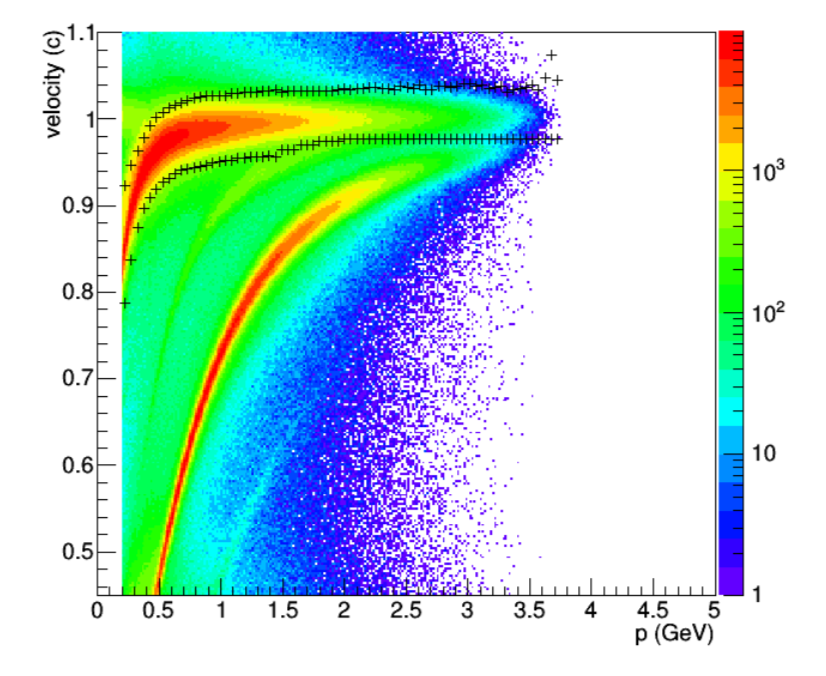
\includegraphics[width=\textwidth]{image/plots/sidis/nathan-pip.png}
  \caption[PID for $\pi^+$ used for the SIDIS analysis]{Positively charged $\pi$ mesons are identified by applying cuts to the momentum dependent $\beta$.}
\end{figure}

In order to determine the cut boundaries, the events are fit with an unnormalized Gaussian distribution in each of 70 momentum bins and the mean $\mu$ and standard deviation $\sigma$ are recorded.  Pions which fall between $\mu - 3\sigma \leq \beta \leq \mu + 3 \sigma$ are kept for analysis.  At higher momentum positive pi-mesons are difficult to separate from protons than at lower momentum values.  To accommodate this, the $\sigma$ value is reduced after 2 GeV.  \\

\begin{table}
	\label{table:hadron-id-nathan}
  \centering
  \begin{tabular}{c|c|c}
    Hadron & $p_{min}$ (GeV) & $p_{max}$ (GeV) \\
    \hline 
	\pi^+ & 0.2 & 3.75 \\
	\pi^- & 0.2 & 3.25 \\
  \end{tabular}
  \caption[Limits for pion momentum used in fitting $\beta$.]{The limits used for pion momentum used in the fitting of $\beta$ for both charged pi-mesons.}
\end{table} 
 
\section{Event Selection}
The identification of an event which contains a good electron and a good pion ($\pi^{\pm}$) is the first step in selecting SIDIS events from the dataset.  Next, events that meet the working assumption for what constitutes the DIS region ($Q^2 > 1.0 \; GeV^2$ and $W > 2.0 \; GeV$) are selected.  A missing mass cut is used in this analysis to remove low lying exclusive resonances which are not produced by the SIDIS mechanism.  Accordingly it is required that the missing mass $M_X (e p \rightarrow e h X)$ be greater than 1.35 GeV (in the positive channel this excludes the delta resonance).  \\

One additional kinematic restriction is applied at the event selection stage, a cut on the maximum allowable inelasticity $y_{max}$.  Full radiative corrections will be discussed in detail, but this kinematic restriction excludes events which have extremely high values of $Q^2$ and are much more likely to have radiated a photon in the initial or final state.  In this analysis $y_{max} = 0.85$ is used.  

\section{Binning}
Both $\pi^+$ and $\pi^-$ are binned using the same scheme.  The momentum fraction $x$ is divided into five equally sized bins from 0.1 - 0.6.  With the exception of the highest $x$ bin, each is split into two $Q^2$ bins.  This binning scheme for $x-Q^2$ is displayed in figure \ref{fig:kinematics_xq2}.  \\

\begin{figure}
  \centering
  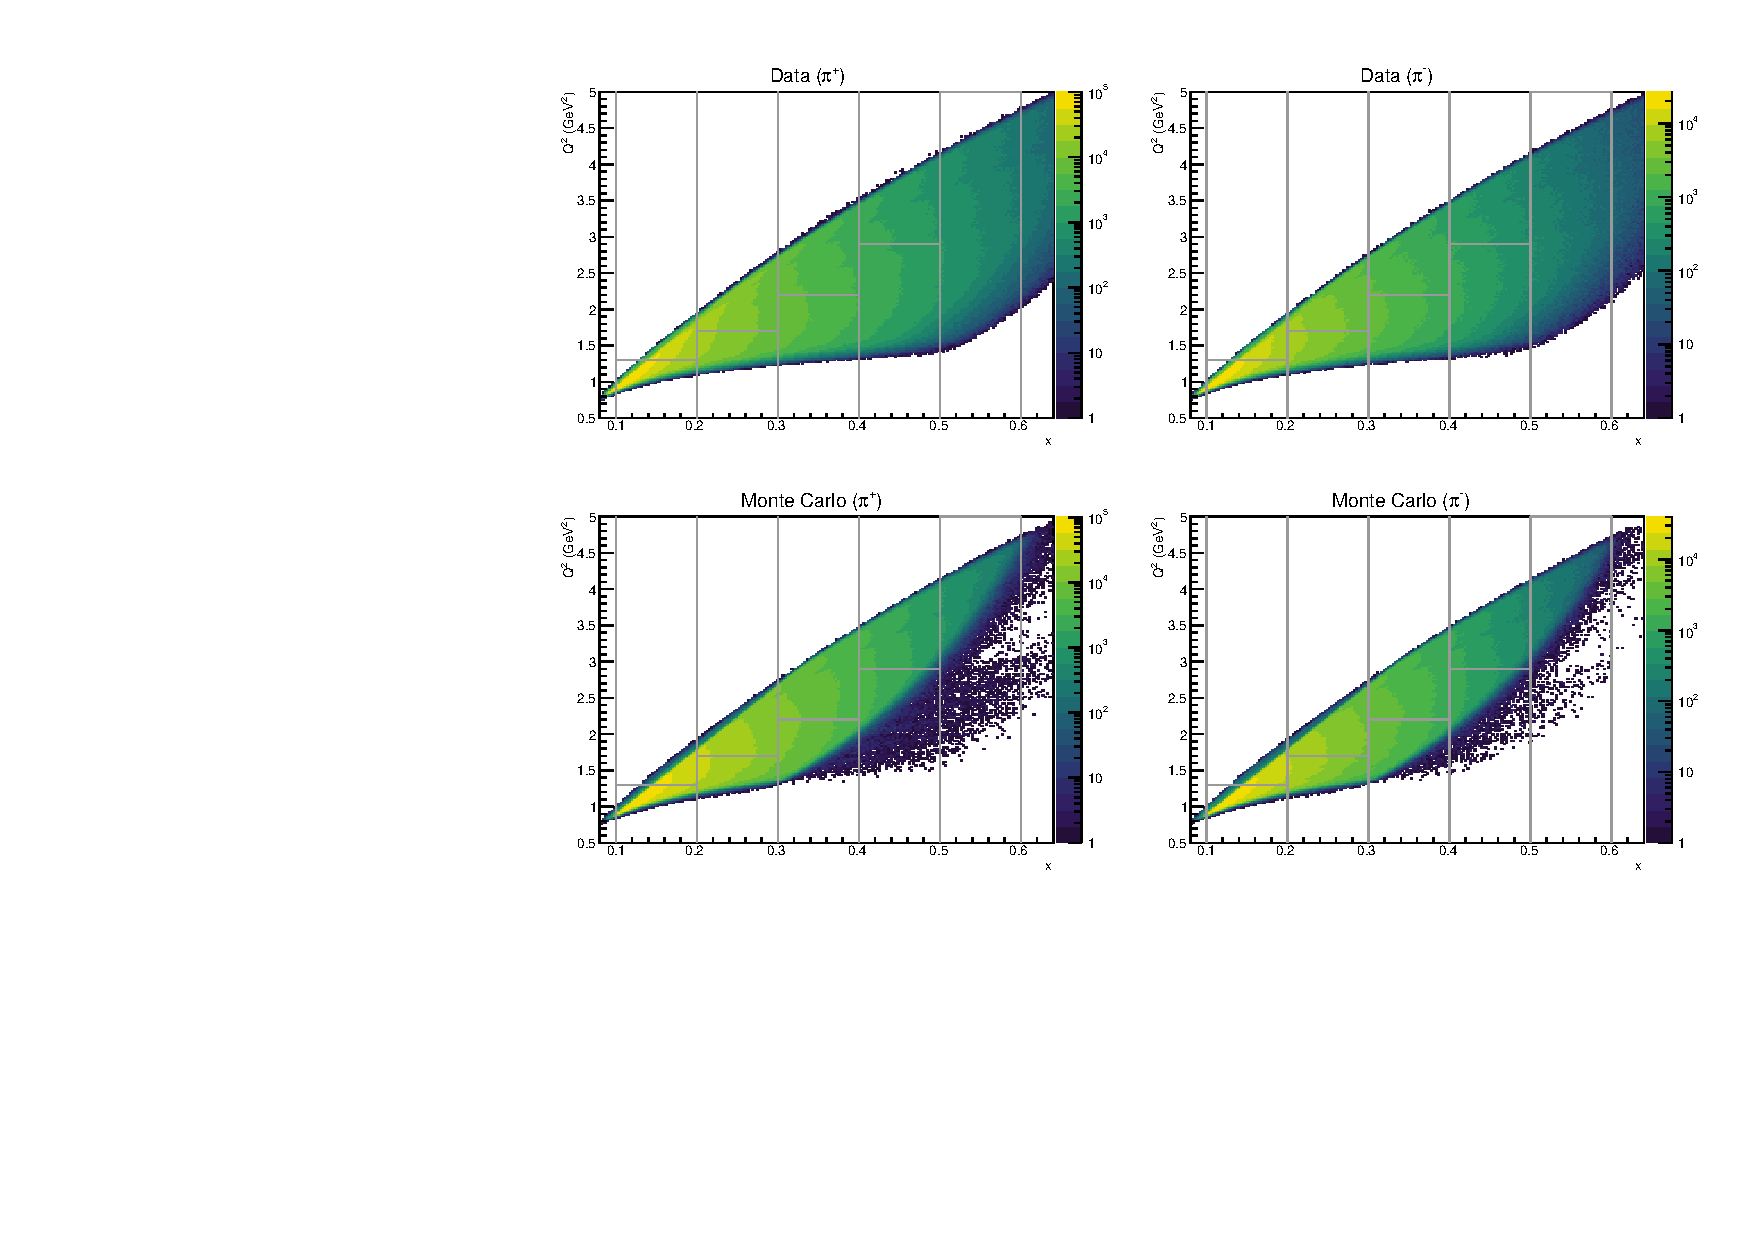
\includegraphics[width=\textwidth]{image/plots/sidis/xq2.pdf}
  \caption[Kinematic distributions and binning for electron variables.]{The kinematic distributions for $\pi^{\pm}$ electron variables shown with binning overlaid.}
  \label{fig:kinematics_xq2}

\end{figure}

\begin{figure}
  \centering
  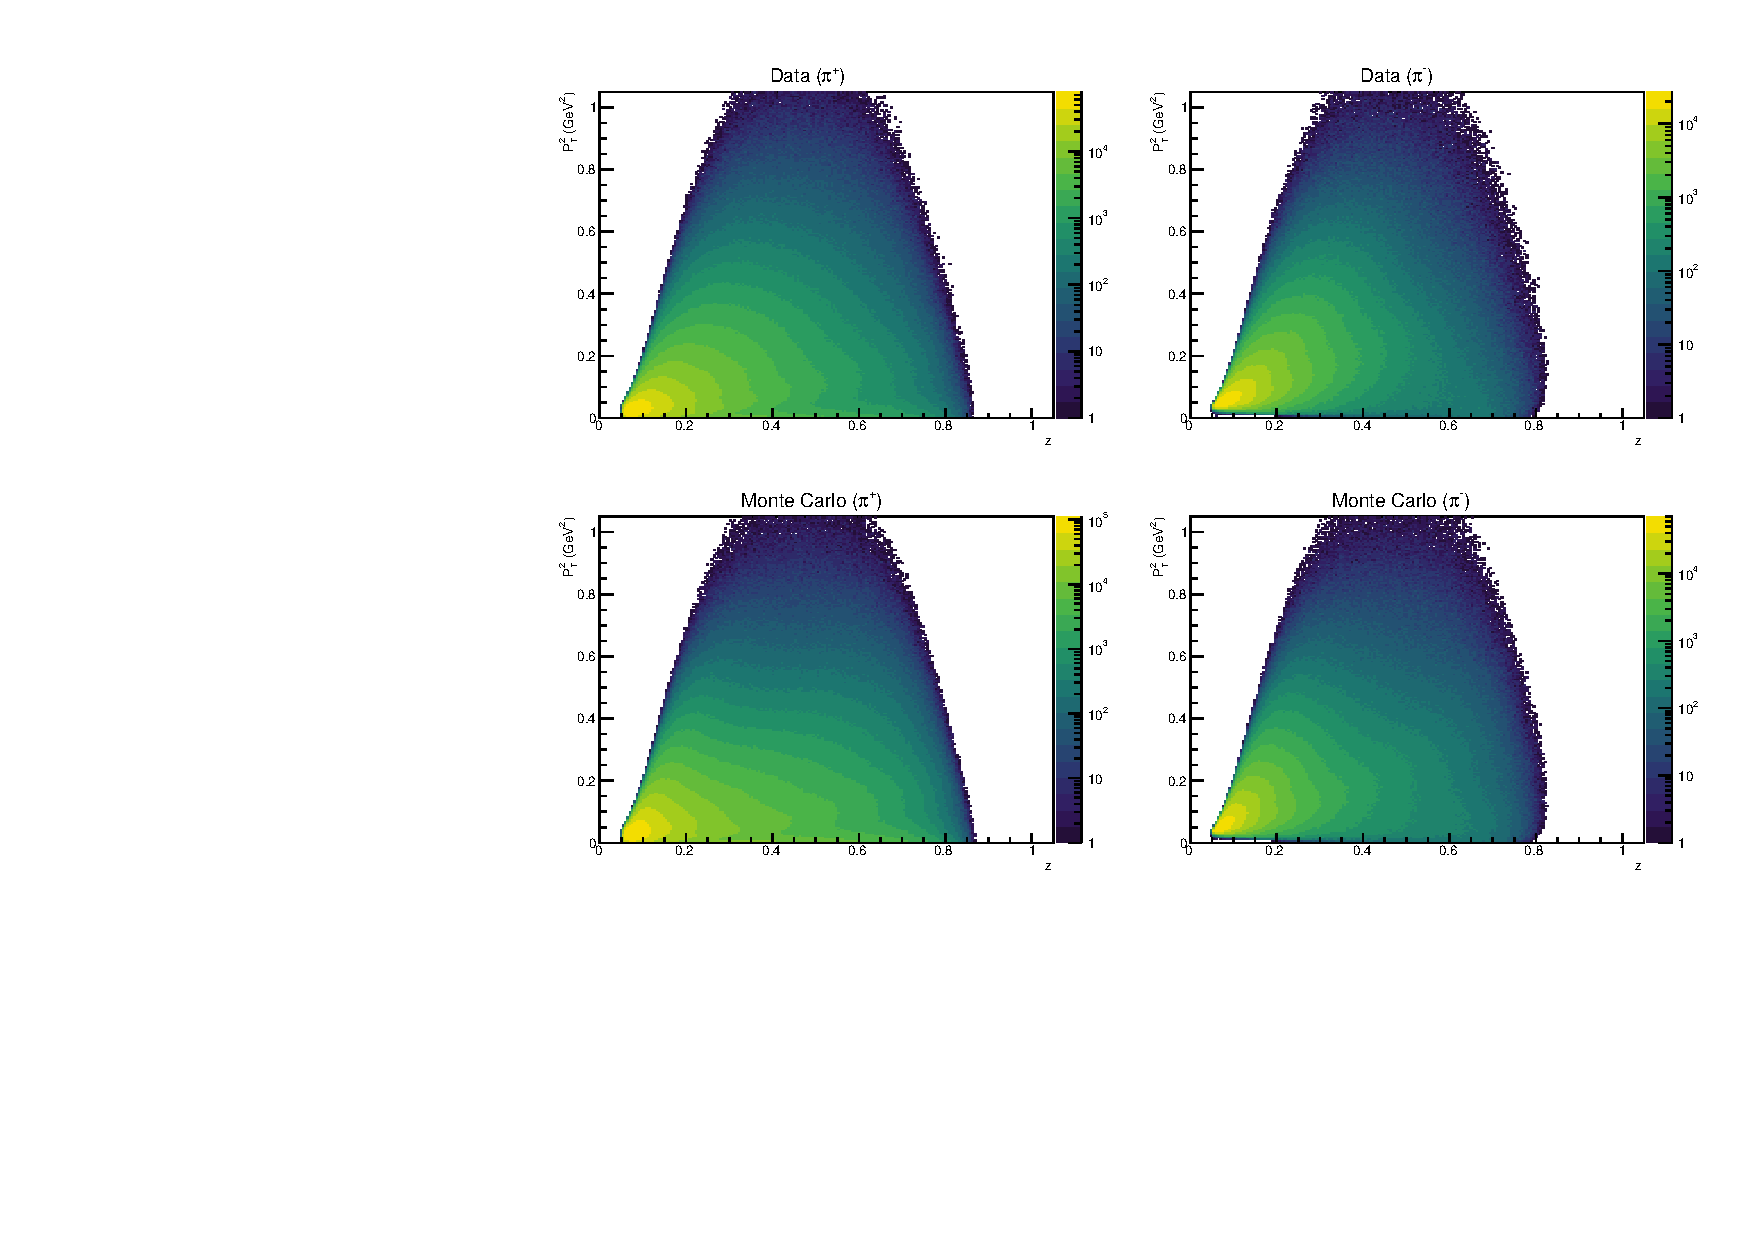
\includegraphics[width=\textwidth]{image/plots/sidis/zpt.pdf}
  \caption[Kinematic distributions and binning for hadron variables.]{The kinematic distributions for $\pi^{\pm}$ hadron variables shown with binning overlaid.}
    \label{fig:kinematics_zpt}

\end{figure}

The hadronic variables are binned finer, the $z$ axis is divided into 18 equal sized bins between 0-0.9, and the transverse momentum squared $P_T^2$ is binned in 20 equally sized bins from 0-1 $GeV^2$.  This simple grid is shown on figure \ref{fig:kinematics_zpt}.  The average value of the kinematic variables in each bin is calculated from the event sample and displayed in the results table at the end of this thesis.

\section{MC Simulation}
Acceptance corrections based on Monte Carlo simulation of the CLAS detector are vital in the accurate calculation of cross sections, and are performed in this work by using a modified version of \texttt{PYTHIA} called \texttt{clasDIS}, the detector simulation \texttt{GSIM}, and the resolution smearing program called \texttt{GPP}.  Two main challenges existed in calculating acceptance corrections for this cross section measurement.  The first challenge, which is common to all acceptance calculations, is that the acceptance depends weakly on the model input used.  The second challenge facing this calculation is that at present the values of the coefficients $A$ which shape the $\phi_h$ distributions are not known, and therefore the events are simulated flat.  \\  

In order to resolve the first challenge, the acceptance model used is included as a source of systematic uncertainty.  This quantifies the amount to which the answer changes based on different input physics models.  In answering the second challenge posed, the model is made more realistic by an iterative procedure of using the extracted $A^{(0)}$ coefficients to weight the generated events and the and produce the coefficients $A^{(1)}$, where the superscript denotes the iteration.  After two iterations, the extracted values of $A$ no longer vary outside of parameter estimation errors.  The last ($2^{nd}$) iteration is used for the simulation of events in this analysis, and the subsequent iteration ($1^{st}$) is used to study systematic uncertainties associated with the difference between both models.  \\

\subsection{Acceptance Corrections}

The generator \texttt{clasDIS} is used with the modified $\phi_h$ dependence and more than 800 million $\pi^+$ events are simulated, as well as more than 600 million $\pi^-$ events.  The acceptance is calculated over the phase space and used to correct the cross section.  A sample of the acceptance is shown in figure \ref{fig:acceptance}.  Two main features are evident, first, the segmented nature of the CLAS detector in the azimuthal direction correlates to the center of mass hadron-electron angle $\phi_h$ and causes a periodic modulation of acceptance.  Additionally, the central region of $\phi_h$ has the lowest acceptance of any value.  For this reason, bins in the central region are excluded if they have large statistical errors from acceptance or have extremely low acceptance values.  The resulting lack of points in the central region impacts the parameter estimation, and is discussed later in the section on parameter estimation.  

\begin{sidewaysfigure}
  \centering
  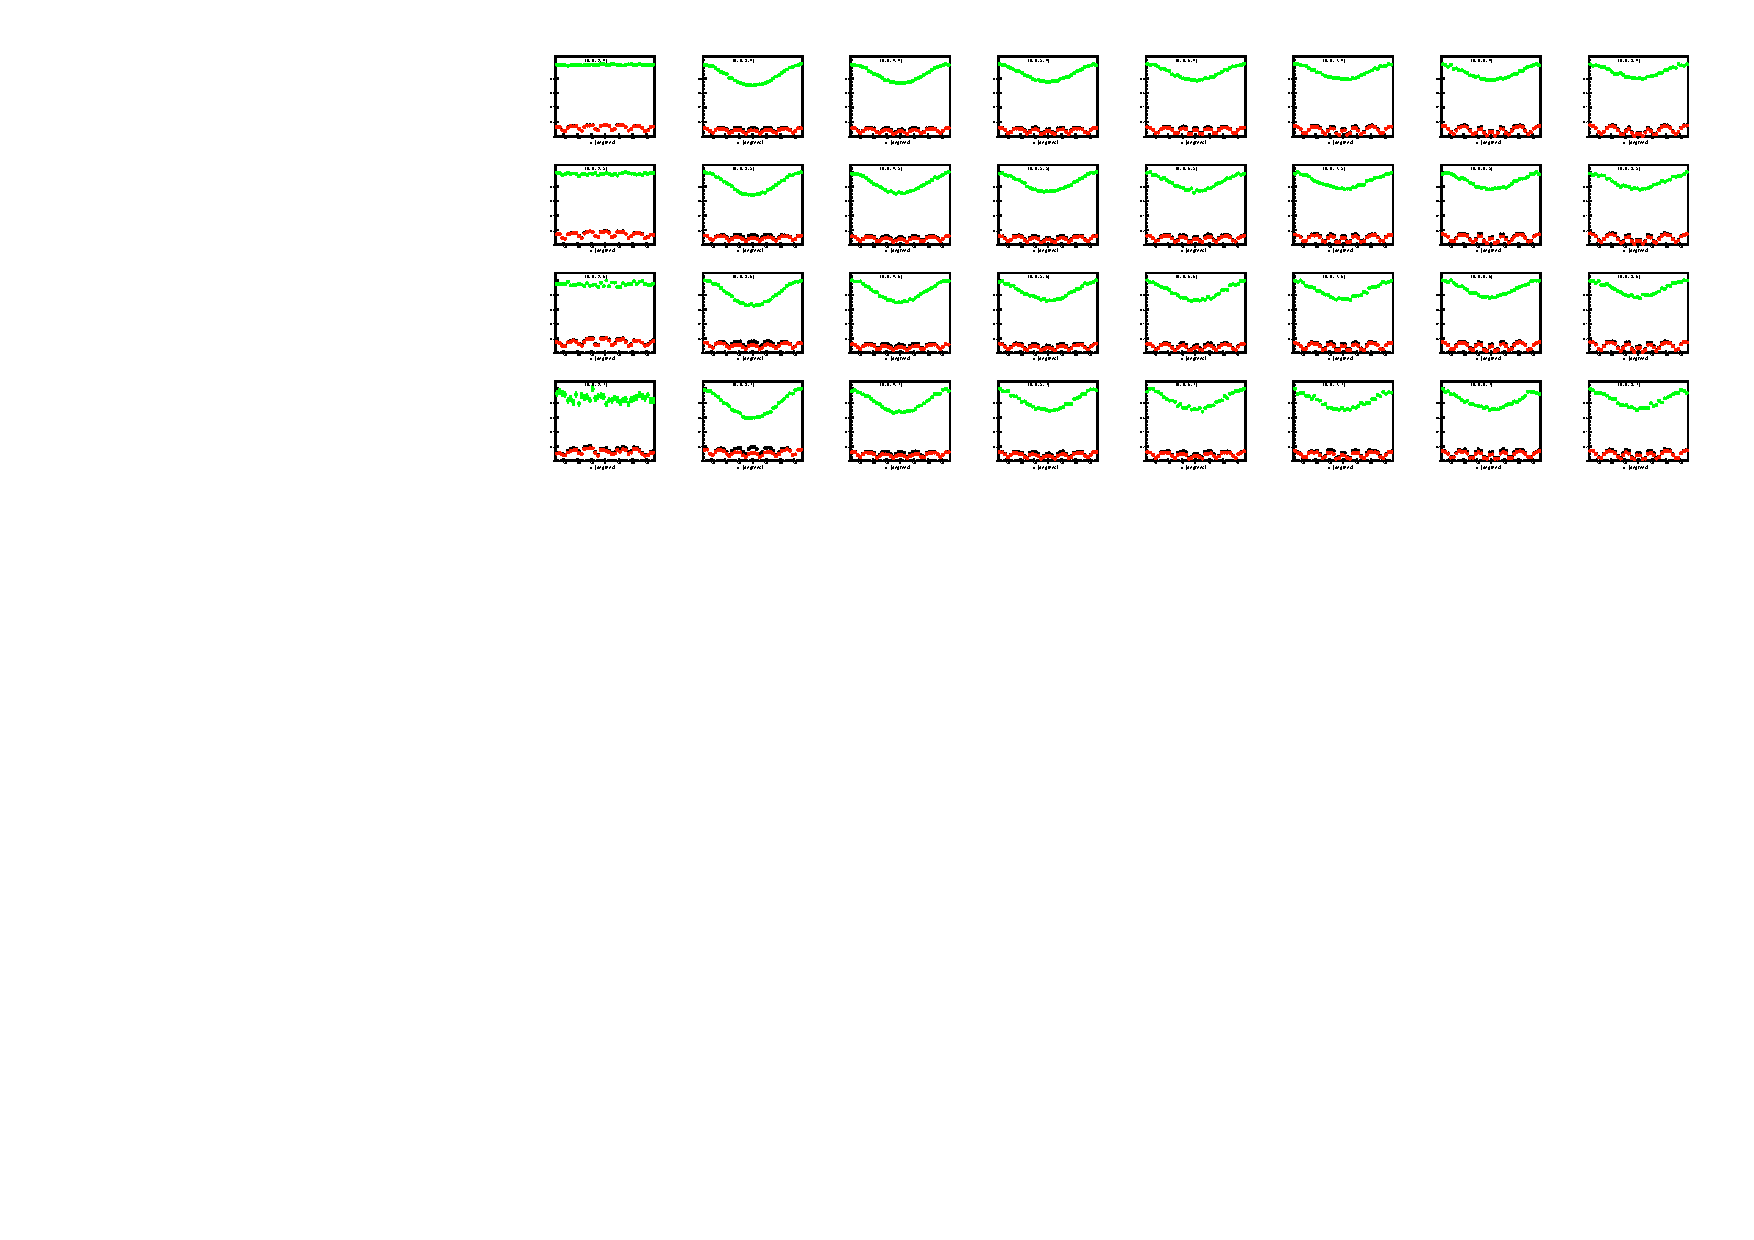
\includegraphics[width=\textwidth]{image/plots/sidis/acceptance.pdf}
  \caption[Acceptance corrections for SIDIS]{Acceptance corrections shown for different $z$ bins (increasing over the horizontal axis) and $P_{T}^{2}$ bins (increasing down the vertical axis) are displayed in red.  Generated events are displayed in green, and in red the reconstructed events are shown normalized by the maximum number of generated events in any bin.  On each figure the complete bin index is given in the format $(x, Q^2, z, P_{T}^{2})$.}
  \label{fig:acceptance}

\end{sidewaysfigure}

\section{Radiative Corrections}

\begin{figure}
	\centering
	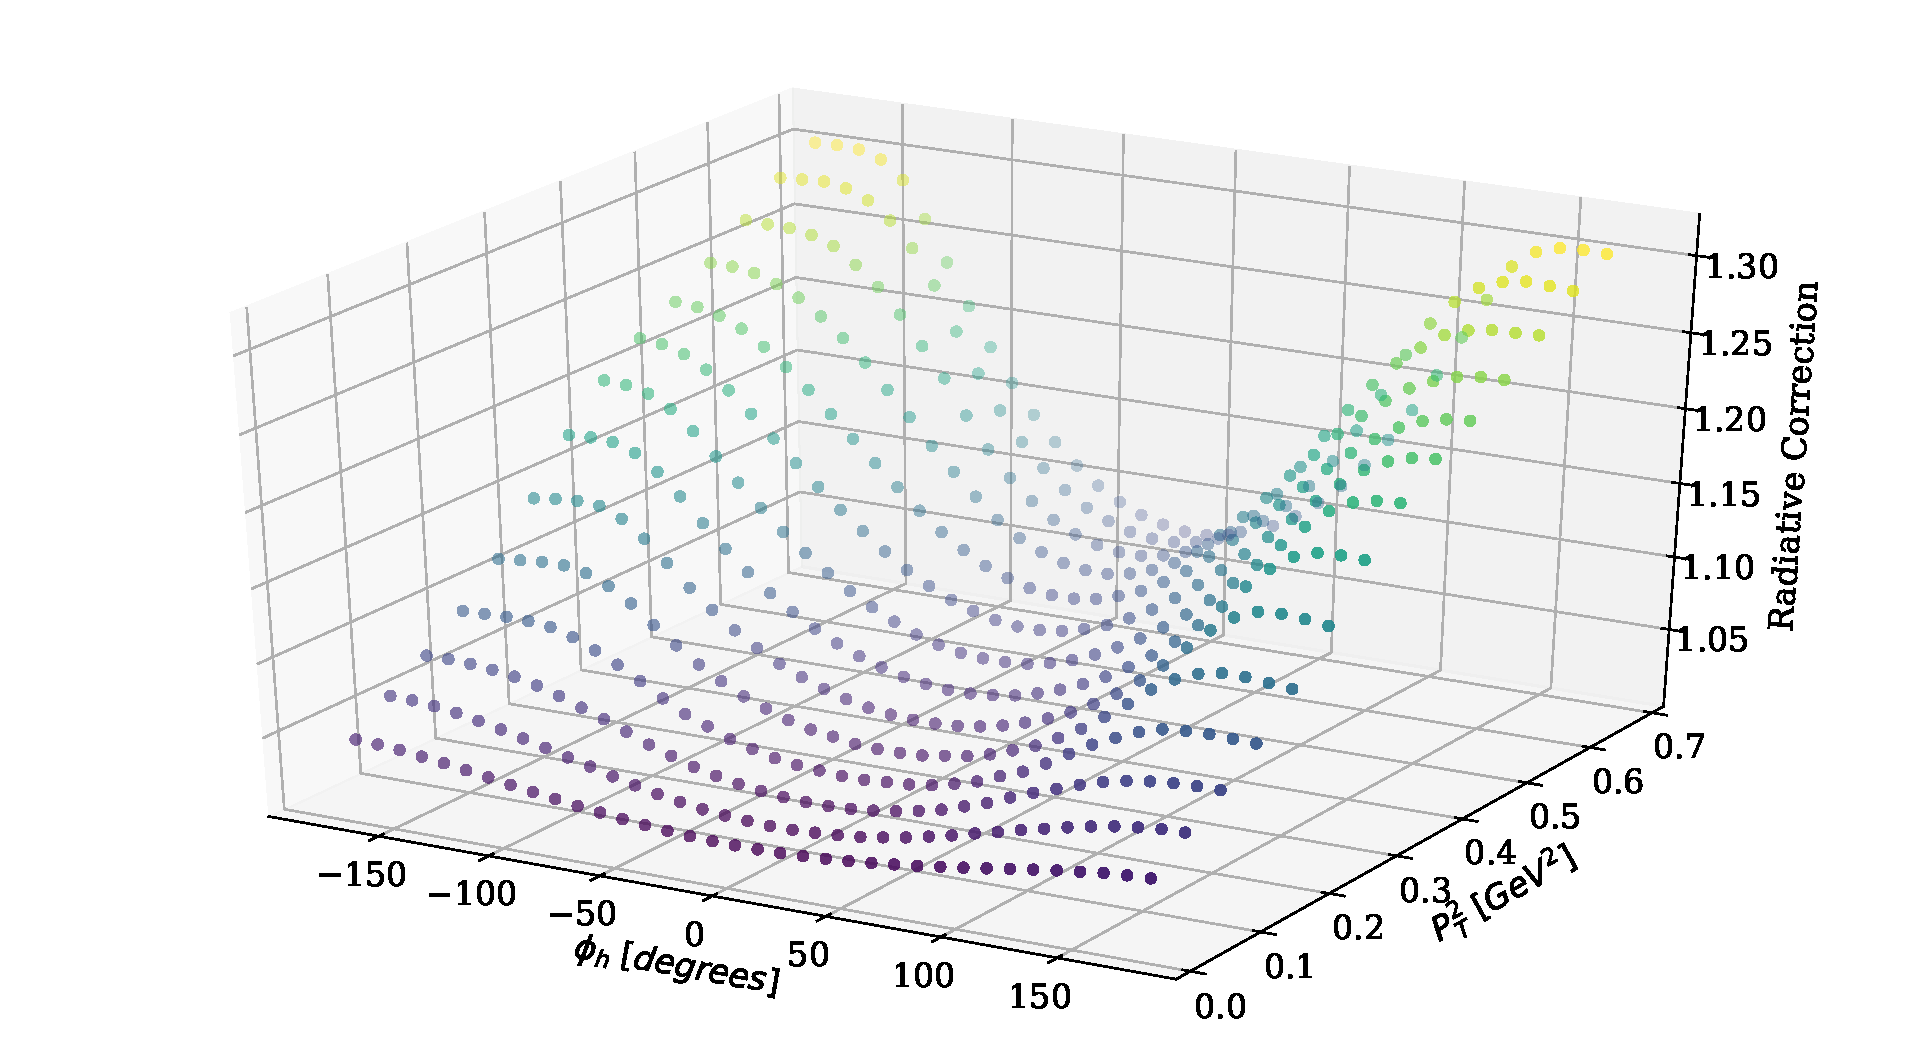
\includegraphics[width=\textwidth]{image/plots/sidis/pip_radcorr.pdf}
	\caption[Radiative corrections for $\pi^+$]{Radiative corrections are displayed as a 3-dimensional scatter plot for the bin with indices ($x = 0, Q^2 = 1, z = 4$) for $\pi^+$.  This correction includes exclusive contributions $\sigma_{tail}$.}
	\label{fig:radcorr-pip}	

\end{figure}

The Born cross section, in which no radiation takes place during the scattering, is the cross section that we intend to measure.  However, the incoming and scattered electron can emit photons, and therefore the cross section measured in the lab is not the Born cross section but the \textit{radiated} cross section.  In addition to initial and final state radiation, radiated exclusive events can have long tails and enter into the SIDIS kinematics.  These effects are calculable by using the software package called \texttt{HAPRAD}, which takes as an input a Born cross section model $\sigma_{Born}$ and produces the radiated version of the cross section. This calculation is performed at each kinematic point that is measured.  \\

\begin{equation}
	\label{eqn:radiative-corr}
	R = \frac{\sigma_{rad} (x, Q^2, z, P_T^2, \phi_h)}{\sigma_{Born} (x, Q^2, z, P_T^2, \phi_h)}
\end{equation}

This software package is used to correct our measured cross section by calculating the ratio $R_{i}$ for each bin i (as shown in equation \ref{eqn:radiative-corr}).  Because the correction depends on the model used, two different models are used and the difference in the extracted structure functions is assigned as a systematic uncertainty in our final analysis.

\section{Parameter Estimation (Fitting)}
Once measurements of the 5-differential corrected yield are made, $\chi^2$ minimization is used to estimate the value of the $A$ coefficients in every bin of ($x, Q^2, z, P_T^2$).  The difference between the data points and the model prediction is called the \textit{residual}, and the square sum of these residuals is known as the mean squared error.  The $\chi^2$ is a simply extends this by the addition of an error term in the denominator.

\begin{equation}
	\chi^2 = \sum_{i = 1}^{n} \frac{(d_i - t_i)^2}{\sigma_i^2}
\end{equation}  

Here $n$ refers to the degrees of freedom, or the number of data points used in fitting the model parameters.  The \texttt{Minuit} minimization package which is included in CERN's ROOT is used to minimize the $\chi^2$ function for each bin and provides the parameters and their associated errors.

\subsection{Minimal Coverage in $\phi_h$ for Fitting}
As points are removed from the central $\phi_h$ region, fitting becomes less stable.  This is particularly problematic as the periodicity of the function increases.  Because the central region of $\phi_h$ has been removed in some cases due to low acceptance, this problem needs to be addressed before the fitting algorithm is applied to all the kinematic bins.  \\

In order to alleviate this concern, the bins of ($x, Q^2, z, P_T^2$) that have a gap from $\Delta \phi_h > 60^{\circ}$ are not fit (-30 to 30 or larger).  This value was set by generating psuedo-data with a known $\phi_h$ dependence given in terms of the three $A$ coefficients.  The distribution was fit, and then points were removed and the distribution was fit again.  This was repeated for several different values of $A$, particularly the cosinusoidal terms.  This study is described in detail in \cite{theses-harrison:2015}.

\begin{sidewaysfigure}
	\centering
	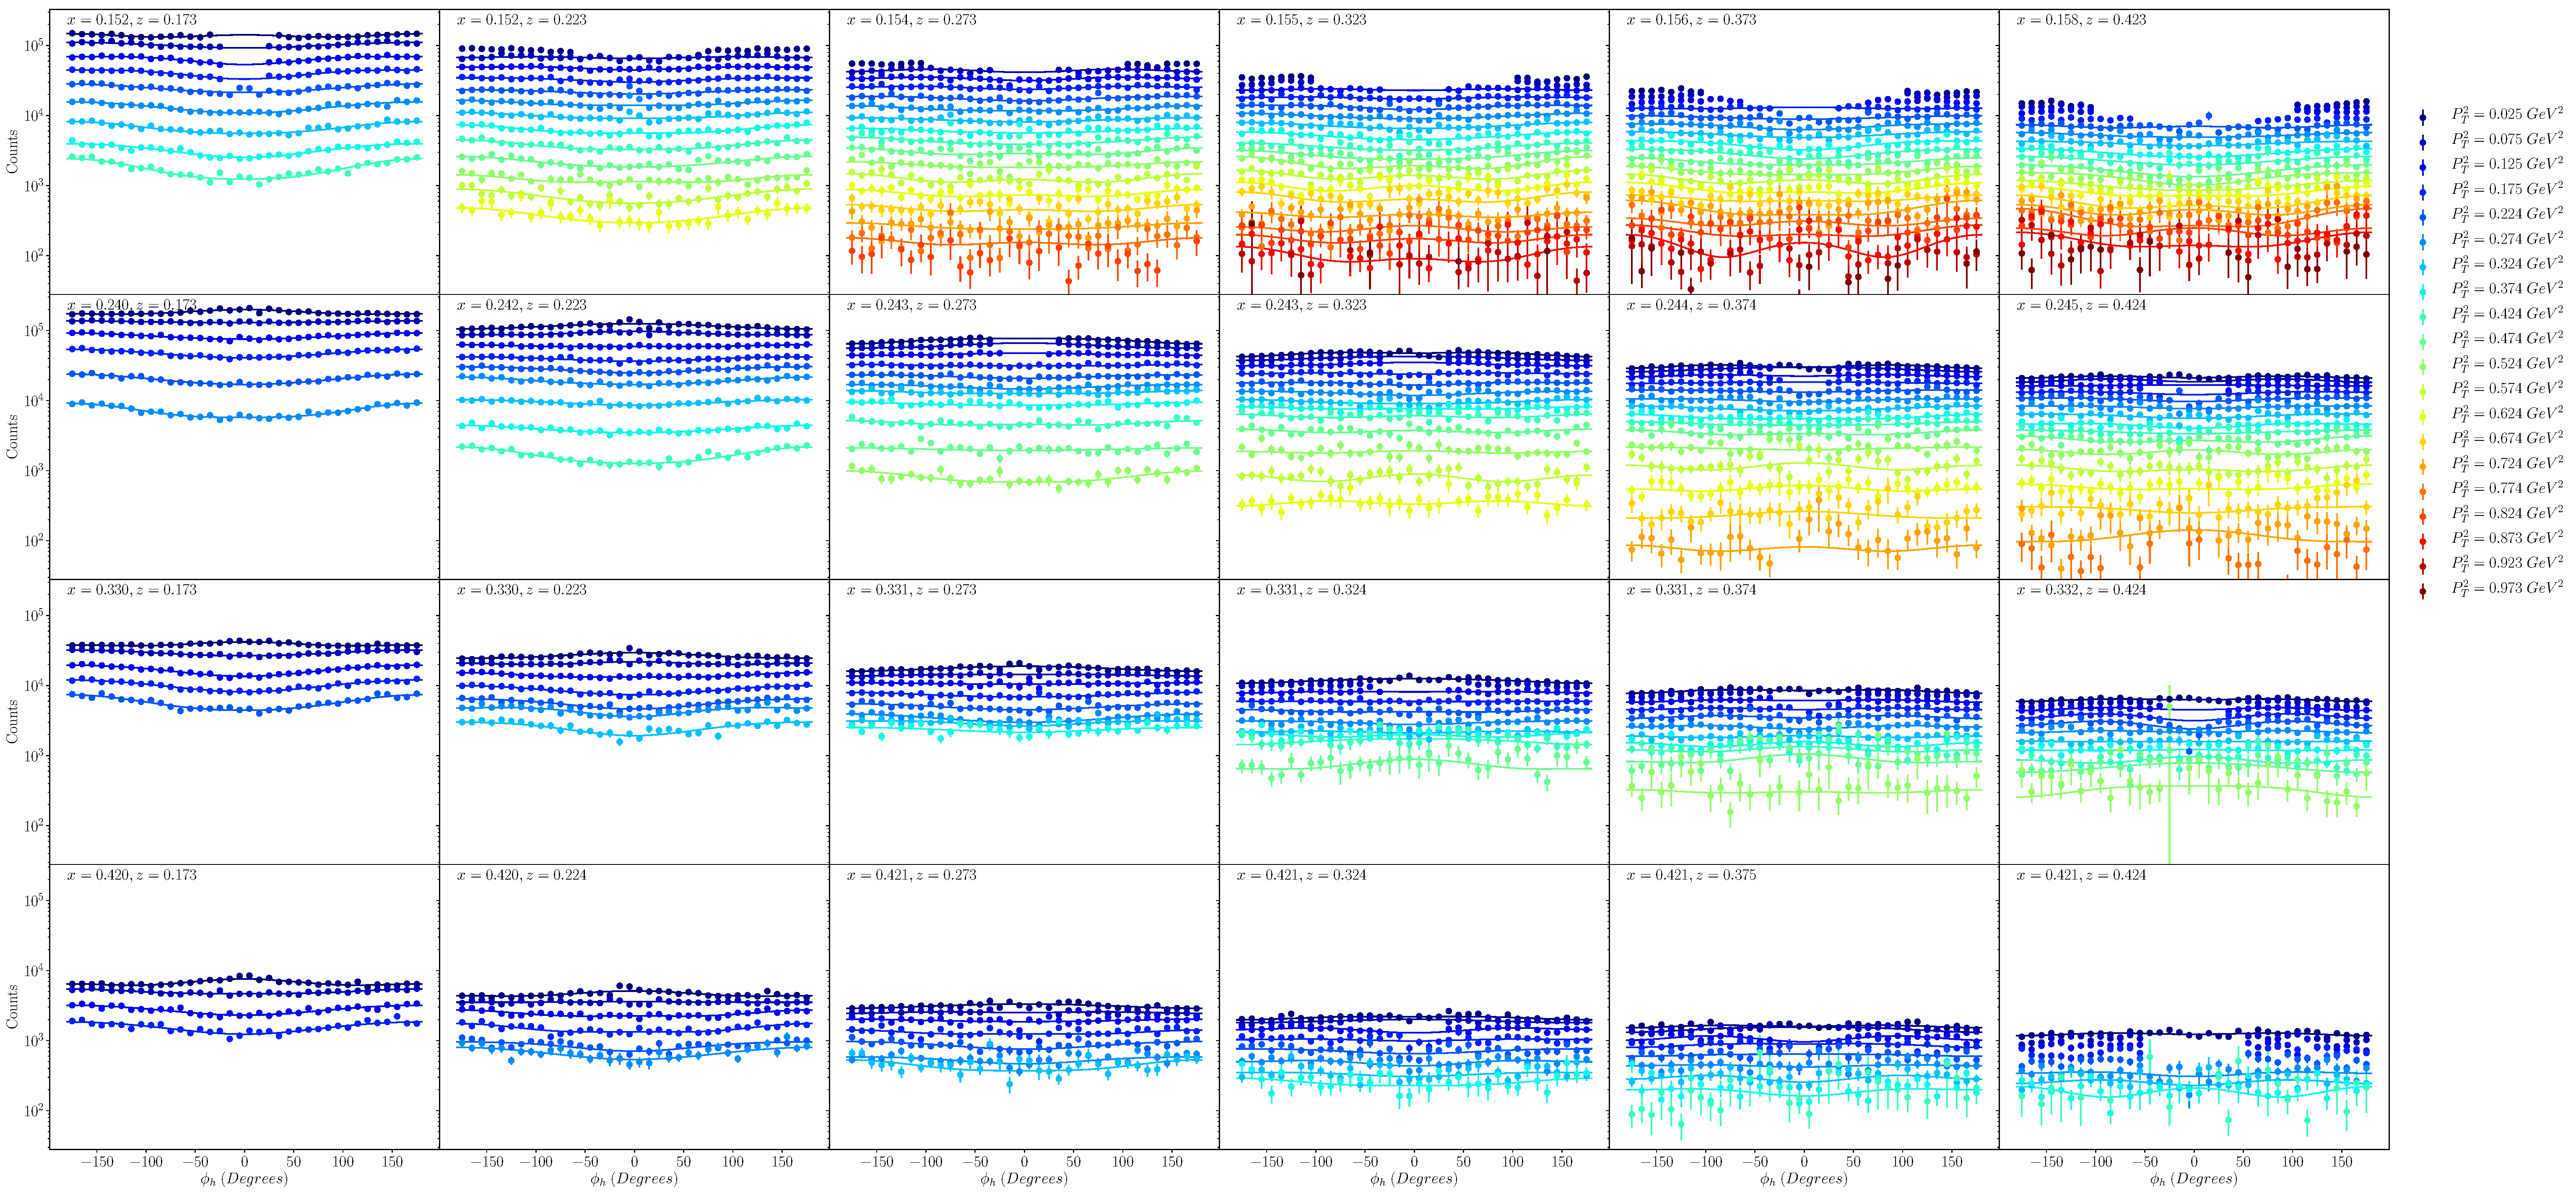
\includegraphics[width=\textwidth]{image/plots/sidis/pip_counts_with_fit_x_z.pdf}	
	\caption[Corrected yield fits for $\pi^+$]{Corrected $\pi^+$ yields are fit and the coefficients $A_{0}$, $A_{UU}^{cos(\phi_h)}$, and $A_{UU}^{cos(2\phi_h)}$ are estimated for each kinematic bin.  In this figure bins of $P_T^2$ are superimposed.  Rows in the figure indicate increasing $x$, while $z$ increases with the column.}
		\label{fig:pip-datafit}

\end{sidewaysfigure}
%	
%	\begin{sidewaysfigure}
%		\centering
%		\includegraphics[width=\textwidth]{image/plots/sidis/pim_counts_with_fit_x_z.pdf}	
%		\caption[Corrected yield fits for $\pi^-$]{Corrected $\pi^+$ yields are fit and the coefficients $A_{0}$, $A_{UU}^{cos(\phi_h)}$, and $A_{UU}^{cos(2\phi_h)}$ are estimated for each kinematic bin.  In this figure bins of $P_T^2$ are superimposed.  Rows in the figure indicate increasing $z$, while $x$ increases with the column.}
%			\label{fig:pim-datafit}
%	
%	\end{sidewaysfigure}

\section{Systematic Uncertainties}
Thirteen possible sources of systematic effect have been identified \ref{table:systematic-sources}, and the values for each are varied slightly from the nominal values in order to observe the affect that each has on the final results.  Each of the values is increased and decreased slightly in accordance with the amount of uncertainty that exists around its ideal value.  The uncertainty due to source $i$ is calculated from these variations by calculating the RMS of the deviations, as shown in equation \ref{eqn:rms}.

\begin{equation}
	\Delta^{(i)} = \sqrt{\frac{1}{N_{vars}} \sum_{j = 1}^{N_{vars}} (r^{(0)} - r^{(j)})^2}
	\label{eqn:rms}

\end{equation}

Here $N_{vars}$ is the number of variations performed for source $i$, and $r^{(0)}$ is the measured result with the nominal set of parameters and $j$ is a an index for the sum over variations of this parameter.  For the acceptance and radiative corrections model dependence instead of increasing and decreasing a value the model is changed and these are treated as variations.  \\

\begin{table}
	\centering
	\label{table:systematic-sources}
	
	\begin{tabular}{c | c | c }
	
	Label & Source & Description \\ 
	\hline 
	
	0      & electron z-vertex cut                          & Varied by $\pm$ 0.2 cm on each side \\ 
	1      & electron sampling fraction cut            & shown in figure \ref{fig:systematics-sampling-fraction} \\ 
	2      & electron EC $E_{dep}$ cut                  & $\pm$ 5 MeV \\ 
	3      & electron EC U, V, W cut                       & shown in figure \ref{fig:systematics-ec-fid} \\ 
	4      & electron $\theta_{CC}$ matching cut & Varied by $\pm$ 0.2 cm on each side \\ 
	5      & electron region 1 fid. cut                      & shown in figure \ref{fig:systematics-region1} \\ 
	6      & electron region 3 fid. cut                     & shown in figure \ref{fig:systematics-region3} \\ 
	7      & electron CC fid. cut                              & shown in figure \ref{fig:systematics-cc-fid} \\ 
	8      & pion $\beta$ cut                                   & $\pm$ 0.25 $\sigma$ \\ 
	9      & pion region 1 fid. cut                             & - \\ 
	10    & $\phi_h$ fid. cut                                    & $\pm \k 10^{\circ}$ on each side \\ 
	11     & acceptance model                                & second to last iteration used \\ 
    12     & radiative correction model                   & second to last iteration used \\ 
	
	\end{tabular}		
\end{table}

\begin{sidewaysfigure}
  \centering
  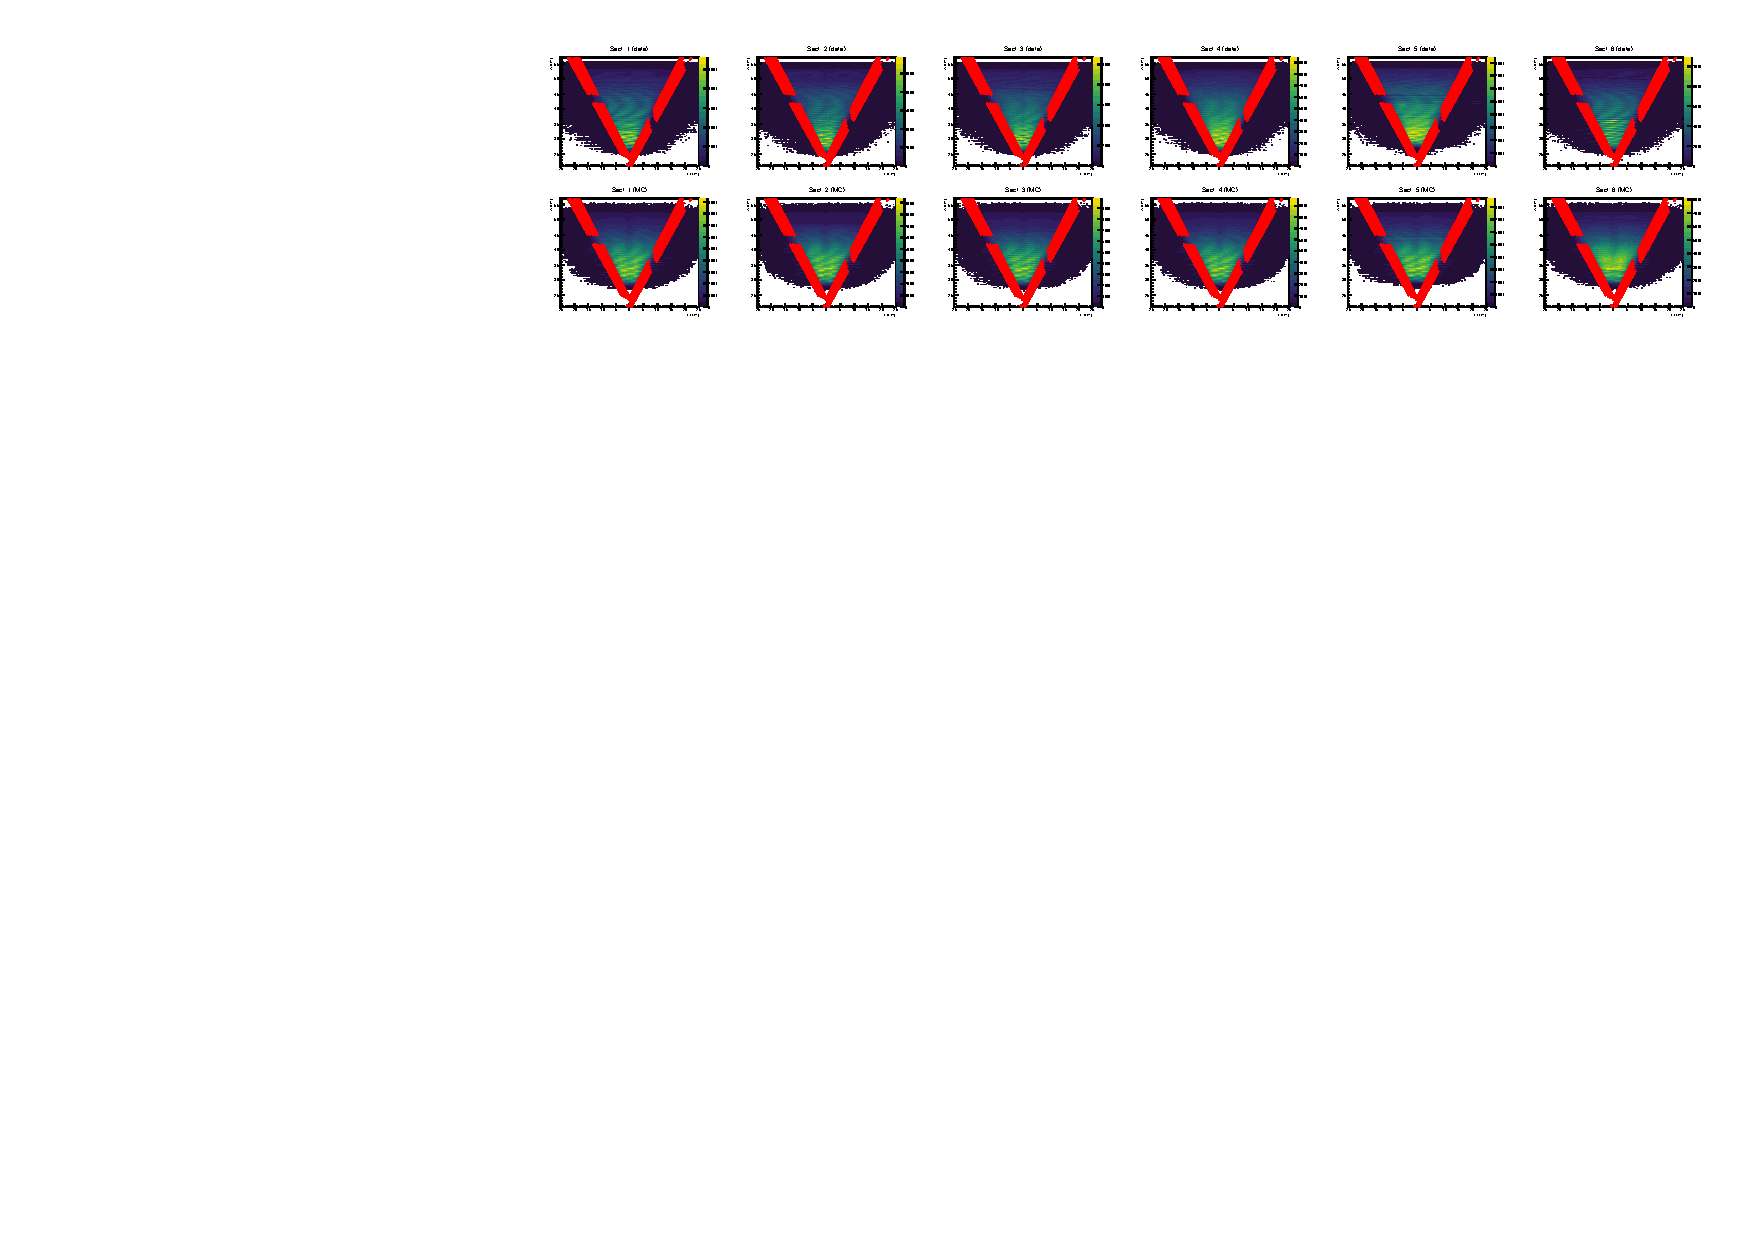
\includegraphics[width=\textwidth]{image/plots/sidis/systematics/region1.pdf}
  \caption[Systematic boundaries on region 1]{Boundaries for electron identification cuts placed on the region 1 drift chambers are shown for data (top row) and Monte Carlo (bottom row).}
    \label{fig:systematics-region1}

\end{sidewaysfigure}

\begin{sidewaysfigure}
  \centering
  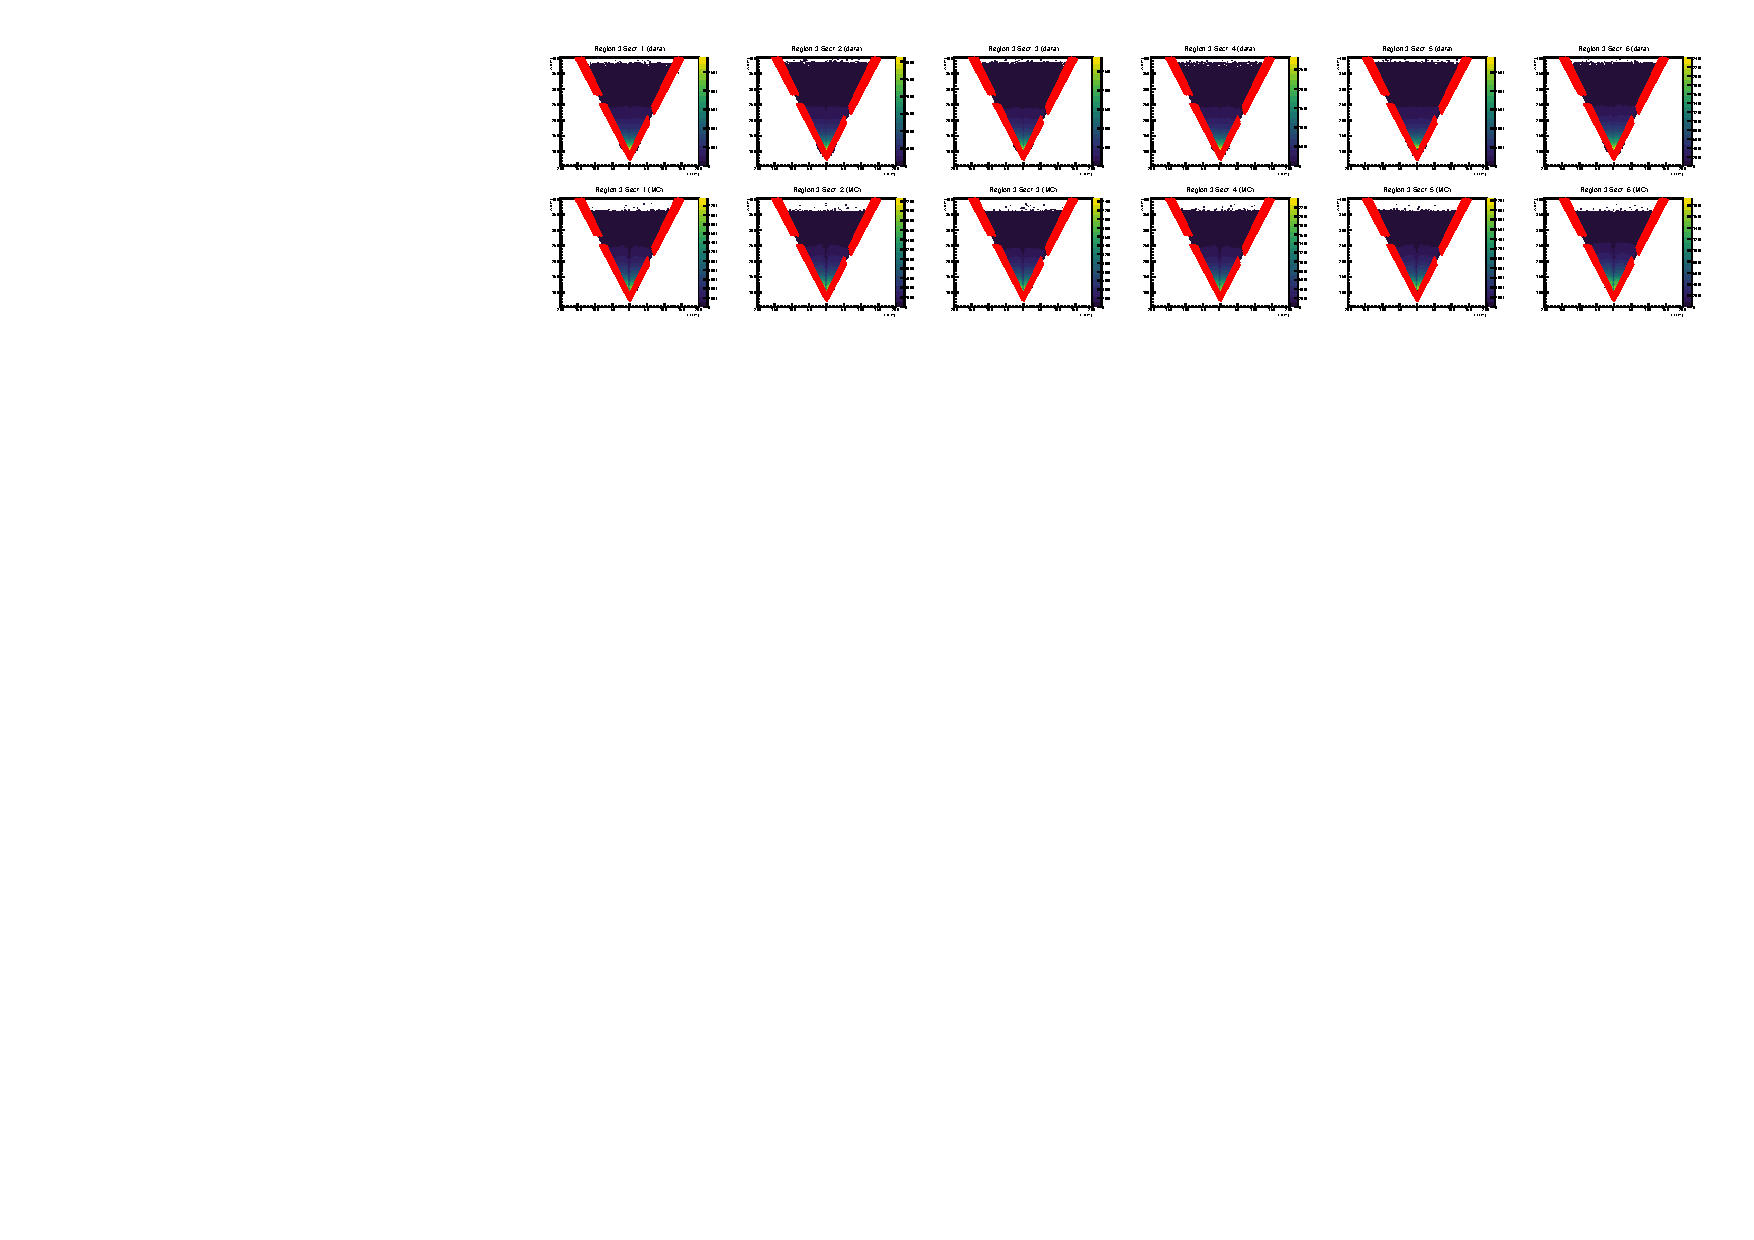
\includegraphics[width=\textwidth]{image/plots/sidis/systematics/region3.pdf}
  \caption[Systematic boundaries on region 3]{Boundaries for electron identification cuts placed on the region 3 drift chambers are shown for data (top row) and Monte Carlo (bottom row).}
    \label{fig:systematics-region3}

\end{sidewaysfigure}

\begin{sidewaysfigure}
  \centering
  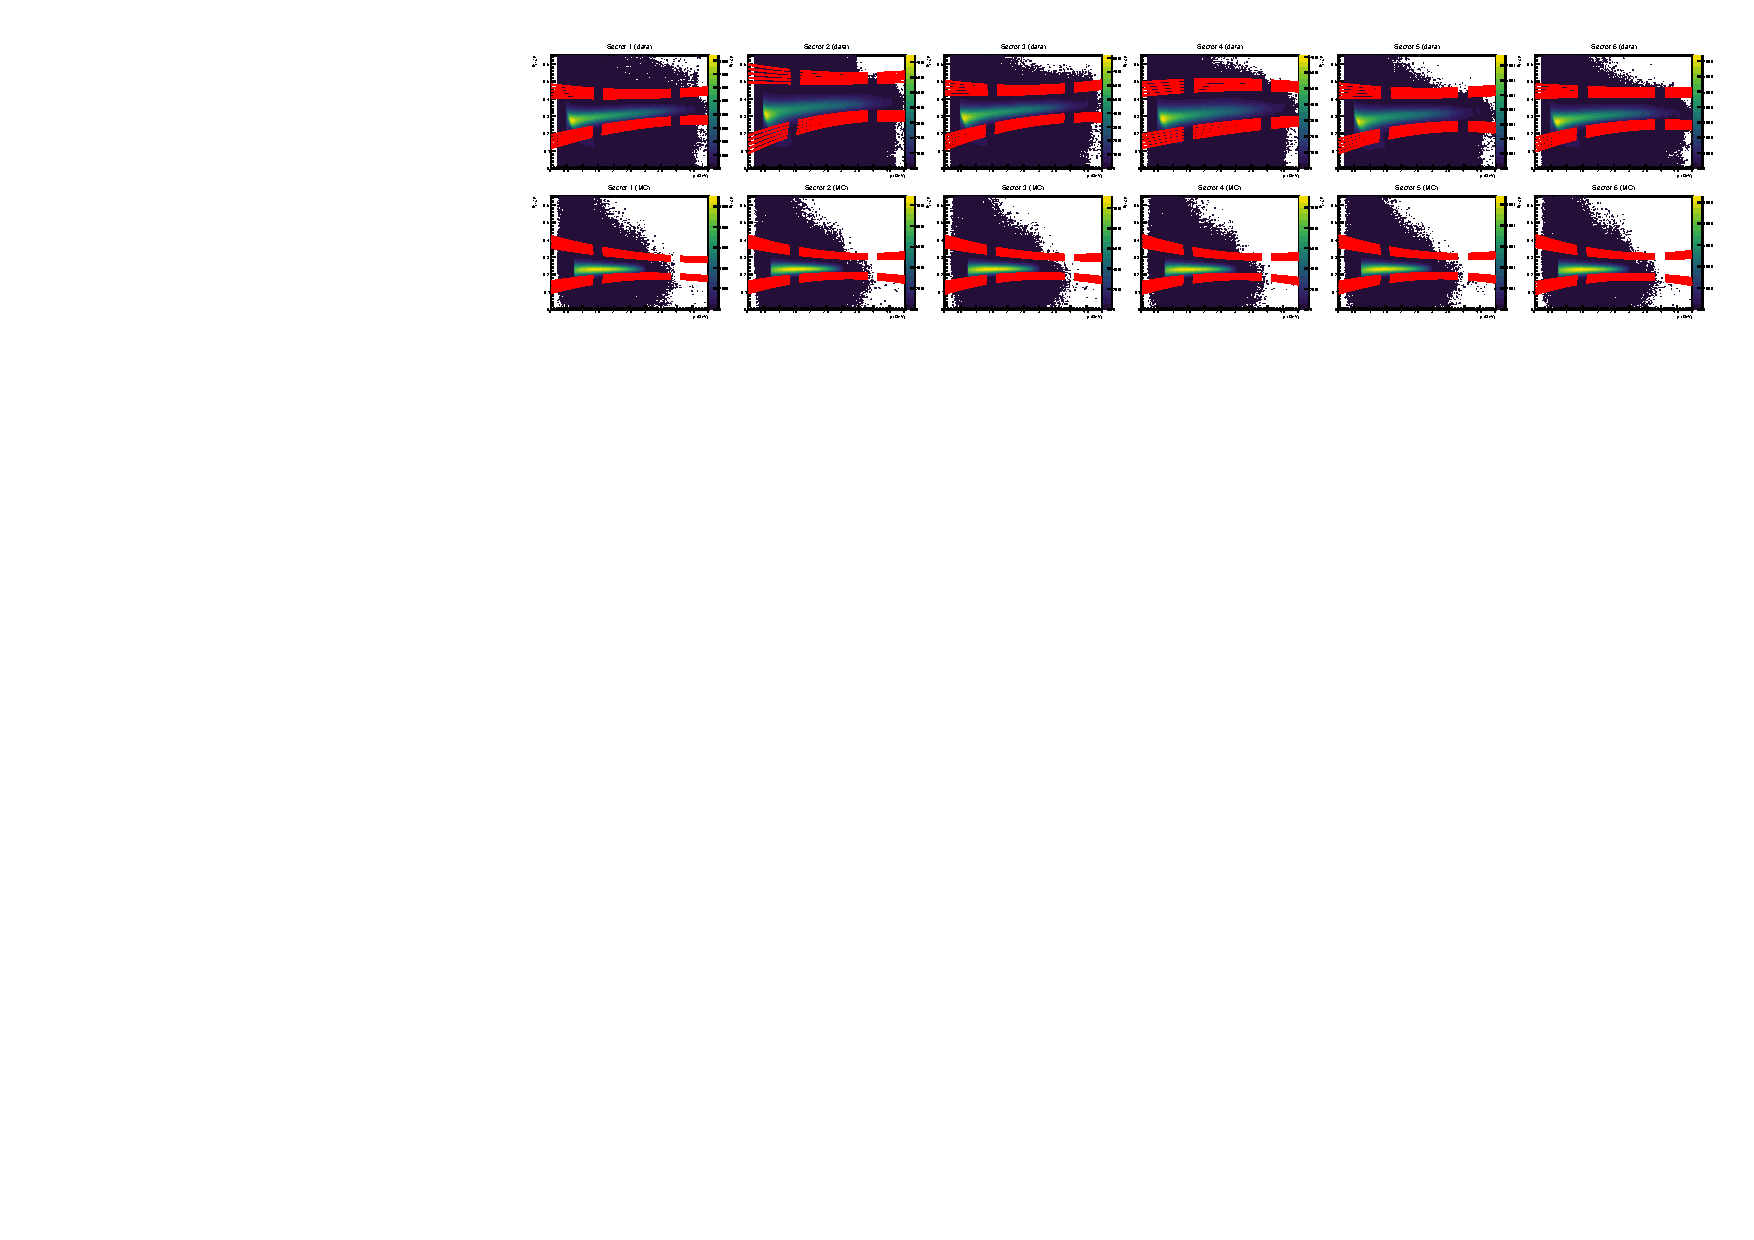
\includegraphics[width=\textwidth]{image/plots/sidis/systematics/sampling_fraction.pdf}
  \caption[Systematic boundaries on sampling fraction]{The sampling fraction boundaries used to identify electrons in data (top) and Monte Carlo (bottom) are shown over the distributions.}
    \label{fig:systematics-sampling-fraction}

\end{sidewaysfigure}

\begin{figure}
  \centering
  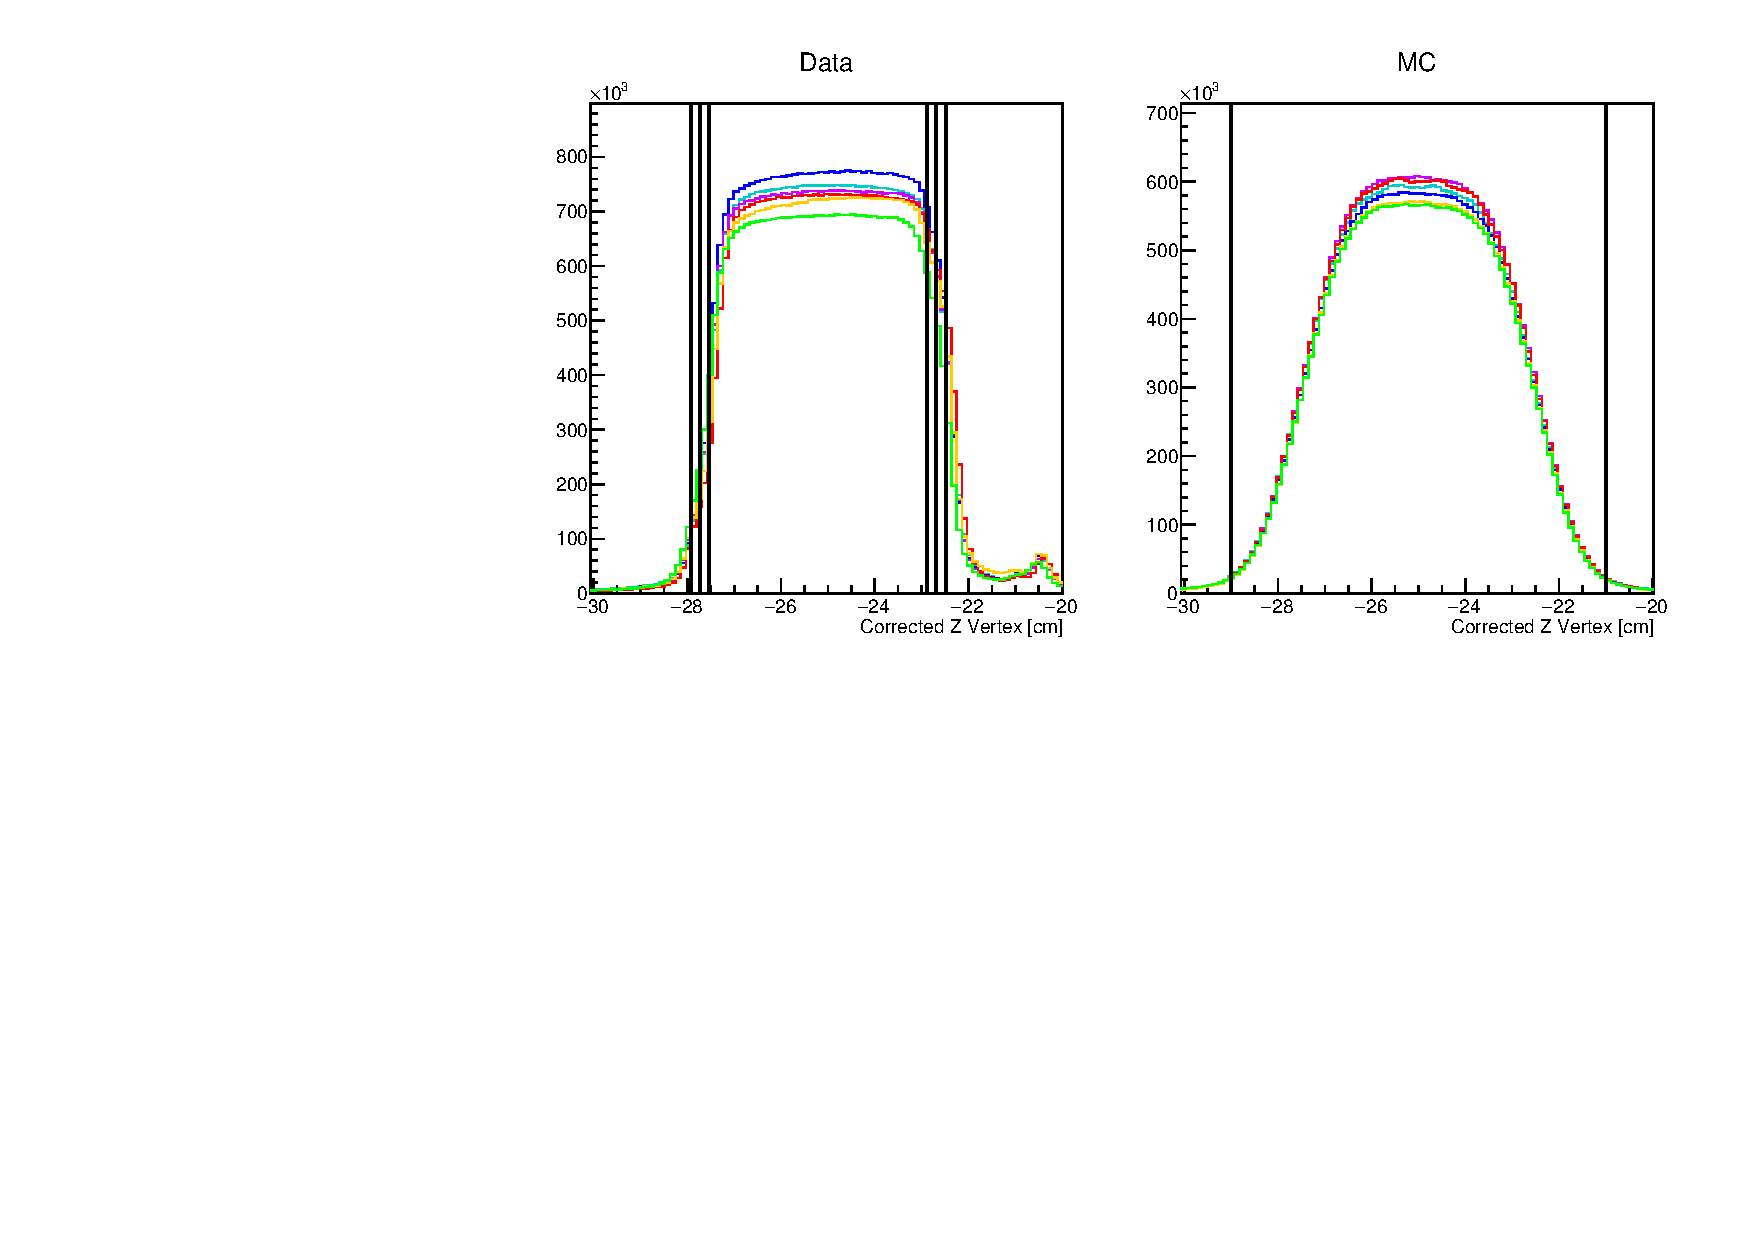
\includegraphics[width=\textwidth]{image/plots/sidis/systematics/z_vertex.pdf}
  \caption[Systematic variations of electron z-vertex cuts.]{The cut boundaries for z-vertex used to identify electrons in data (left) and Monte Carlo (right).  This histograms shown for data have been corrected before being filled.}
    \label{fig:systematics-z-vertex}

\end{figure}

\begin{figure}
  \centering
  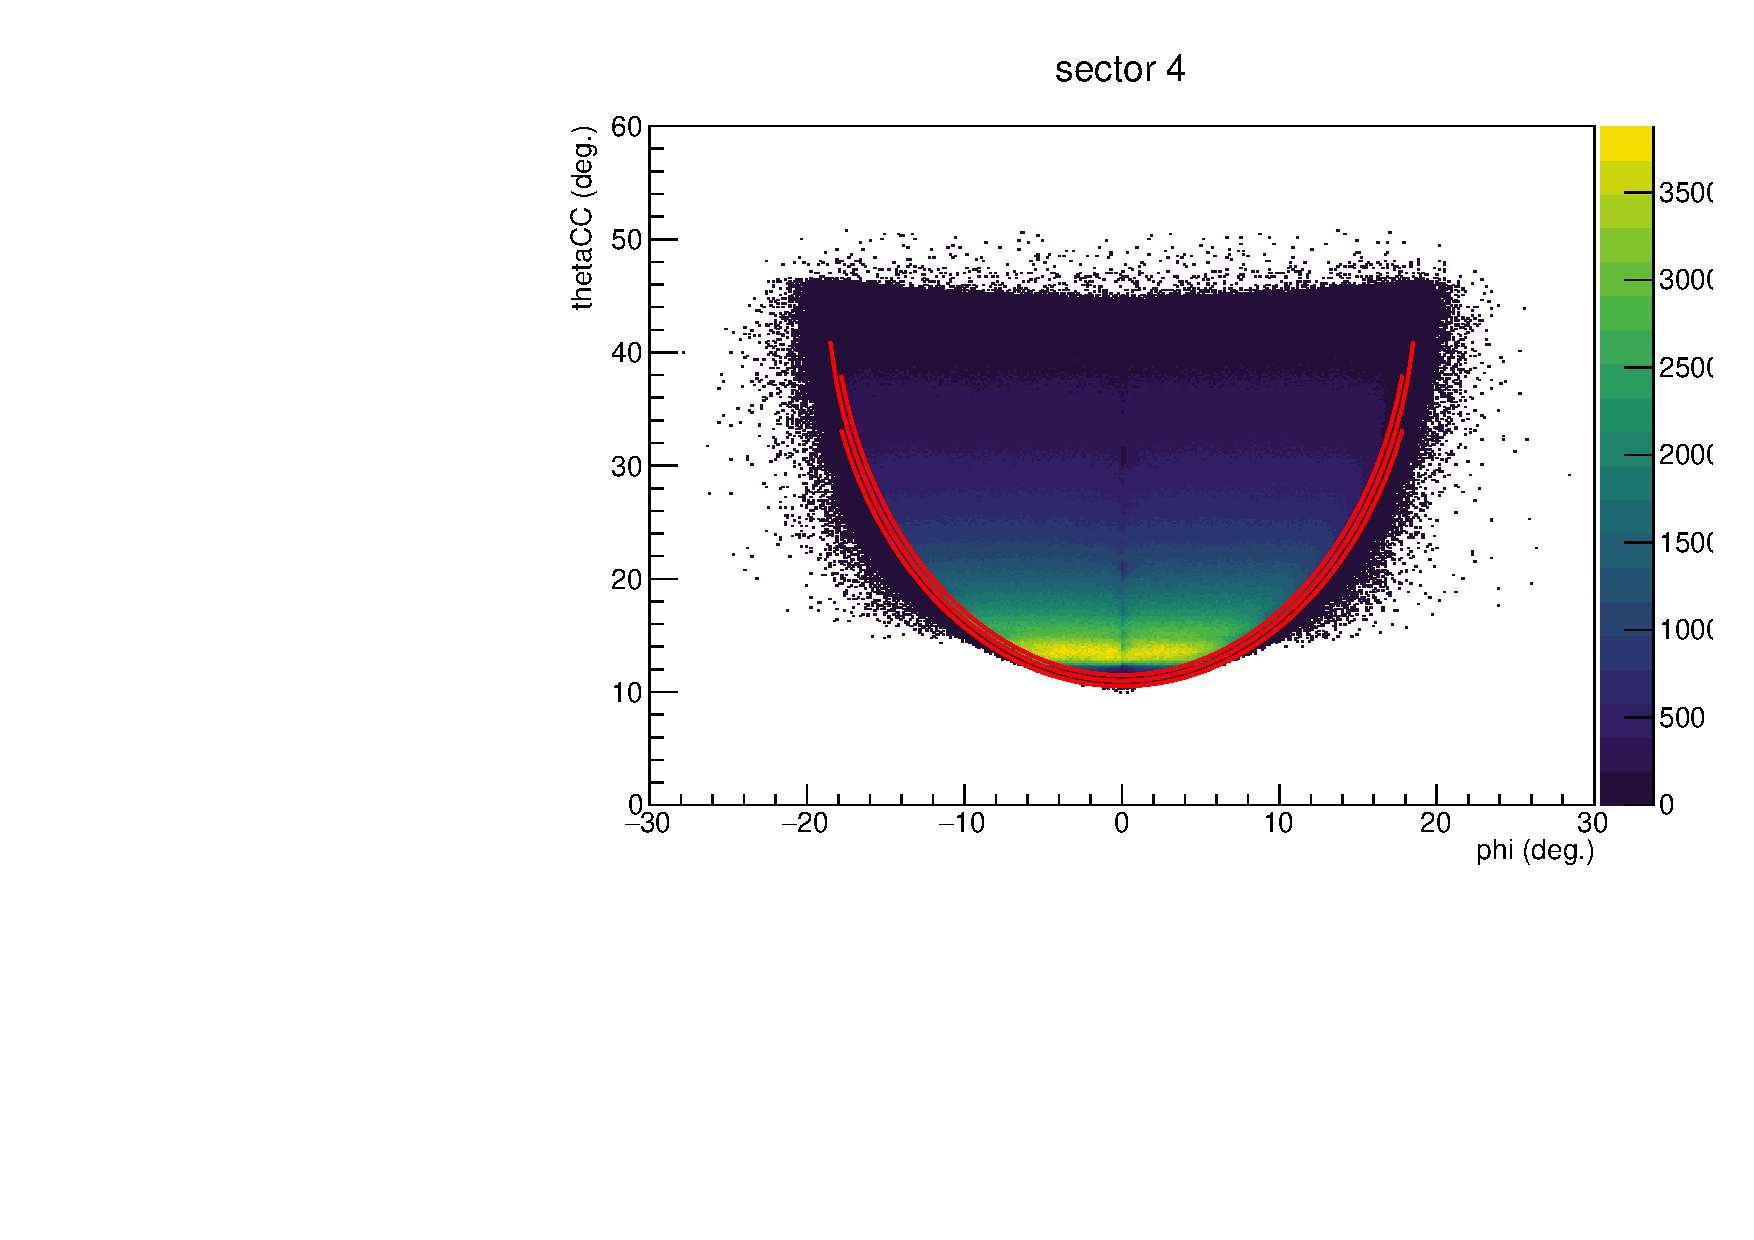
\includegraphics[width=\textwidth]{image/plots/sidis/systematics/cc_fid.pdf}
  \caption[Systematic variations of the CC fiducial cut for electrons.]{The loose, nominal, and tight boundaries applied to data for the fiducial cuts on the Cherenkov Counter.}
    \label{fig:systematics-cc-fid}

\end{figure}

\begin{figure}
  \centering
  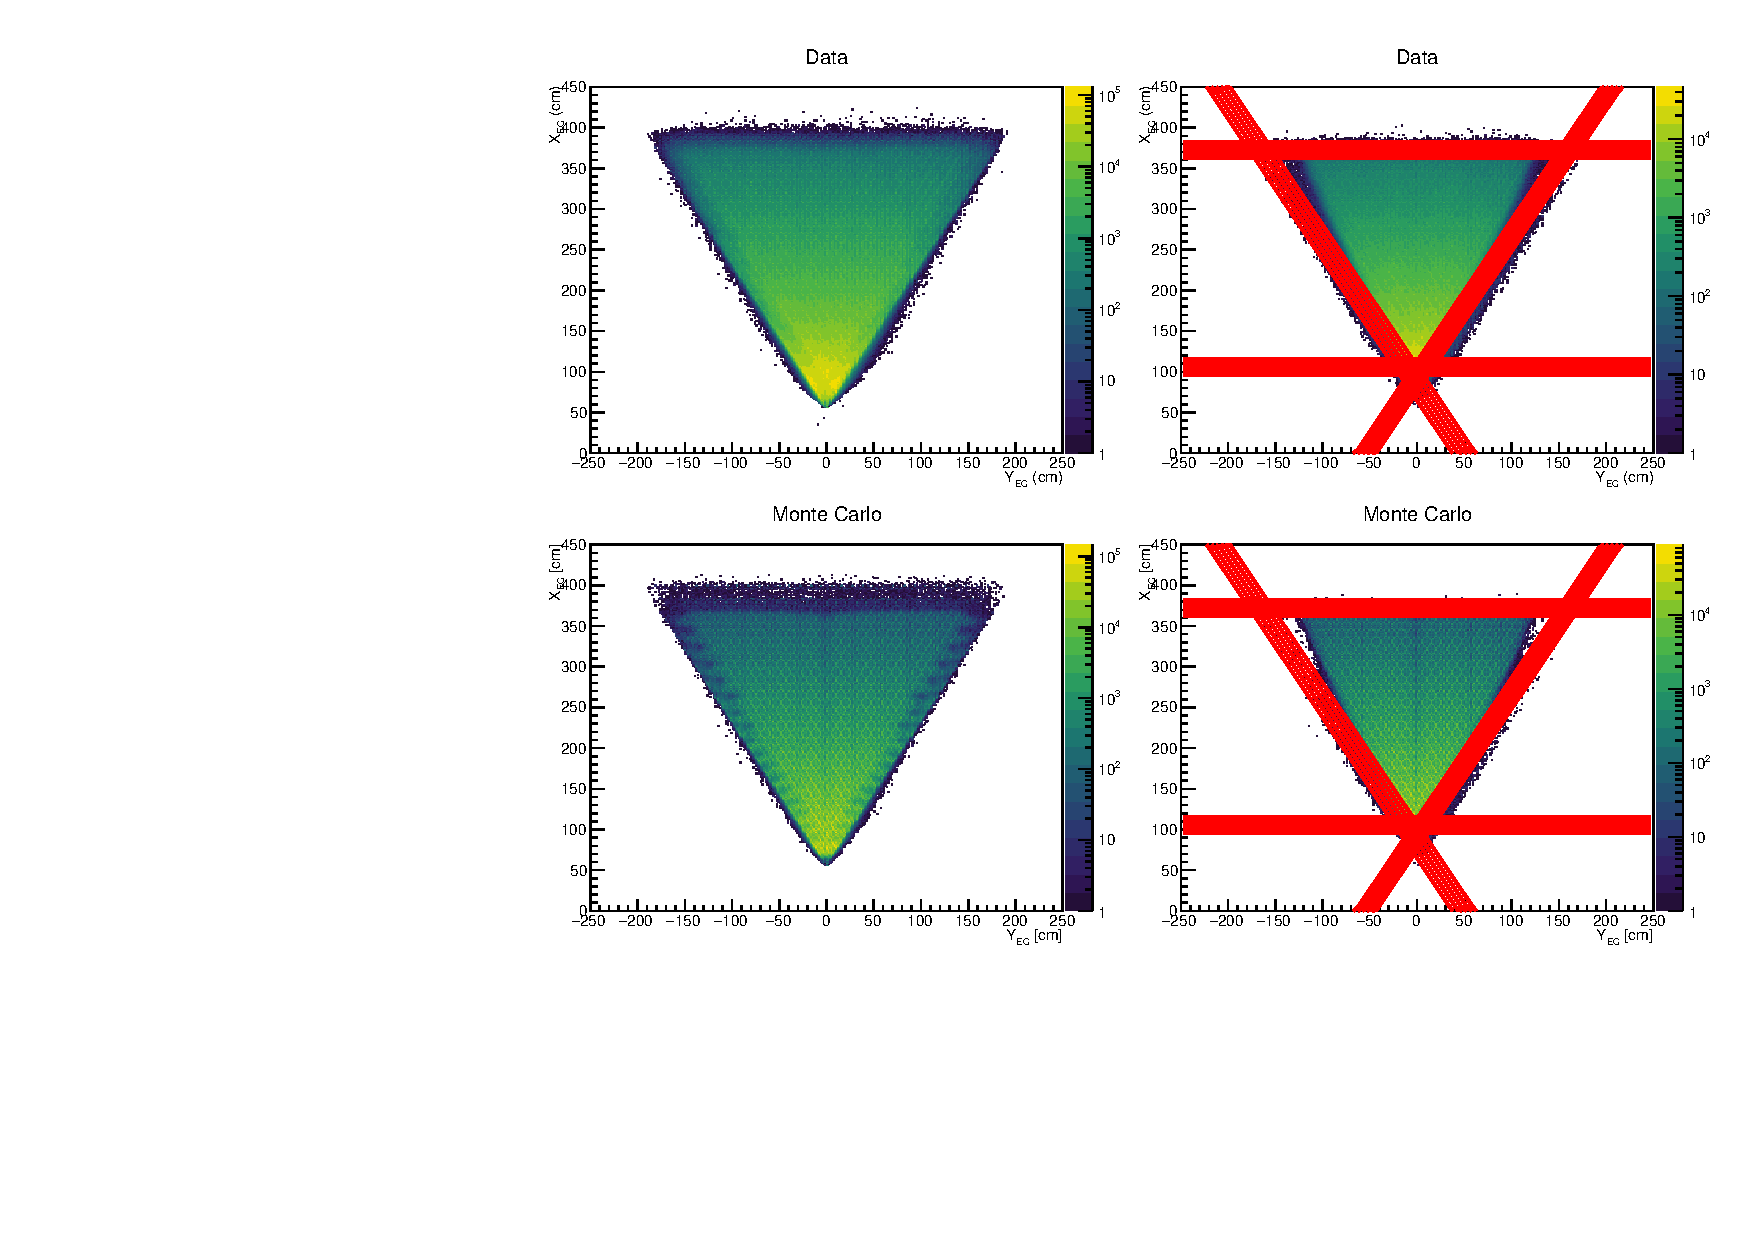
\includegraphics[width=\textwidth]{image/plots/sidis/systematics/ec_fid_sect1.pdf}
  \caption[Variation of EC U, V, and W cuts used to identify electrons.]{Electron identification cuts on U, V, and W coordinates are shown in x-y space.}
    \label{fig:systematics-ec-fid}

\end{figure}

\begin{sidewaysfigure}
  \centering
  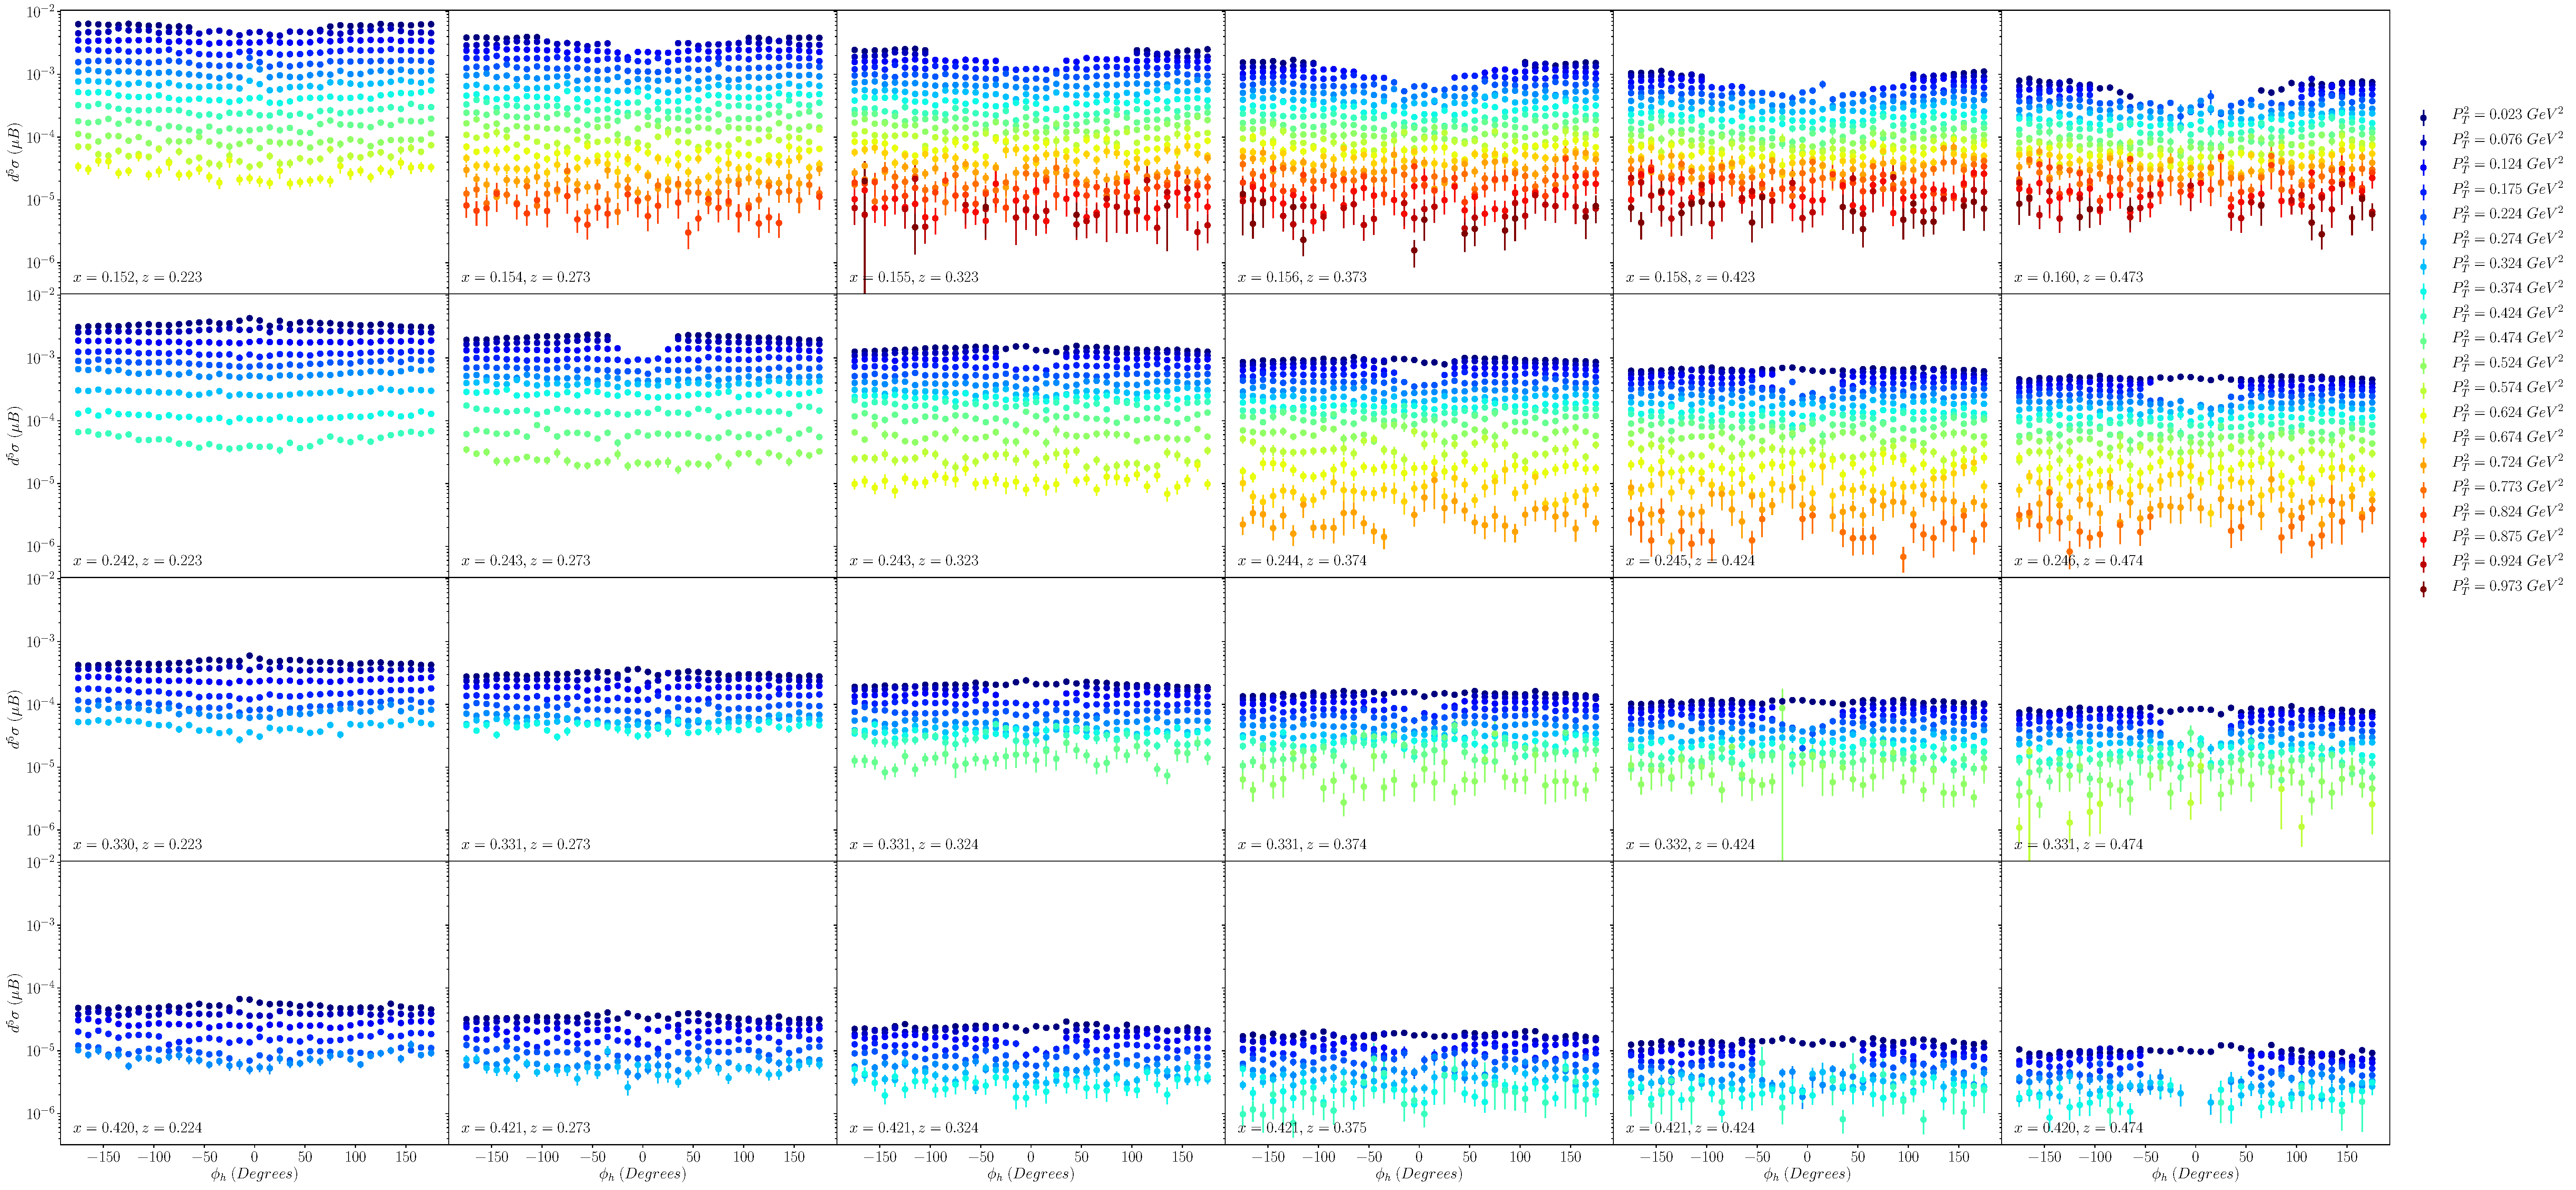
\includegraphics[width=\textwidth]{image/plots/sidis/pip_cross_section_x_z.pdf}
  \caption[$d^5\sigma$ for $\pi^+$]{The 5-differential cross section for $\pi^+$ shown for different values of $x$ and $z$ in different panels of the figure.  In each panel, the $P_T^2$ dependence of the cross section is shown by superimposing different bins in different colors.  The legend at the right of the figure contains information about the colors and their corresponding $P_T^2$ value.}
    \label{fig:cross-section-pip}

\end{sidewaysfigure}


\begin{sidewaysfigure}
	\centering 
	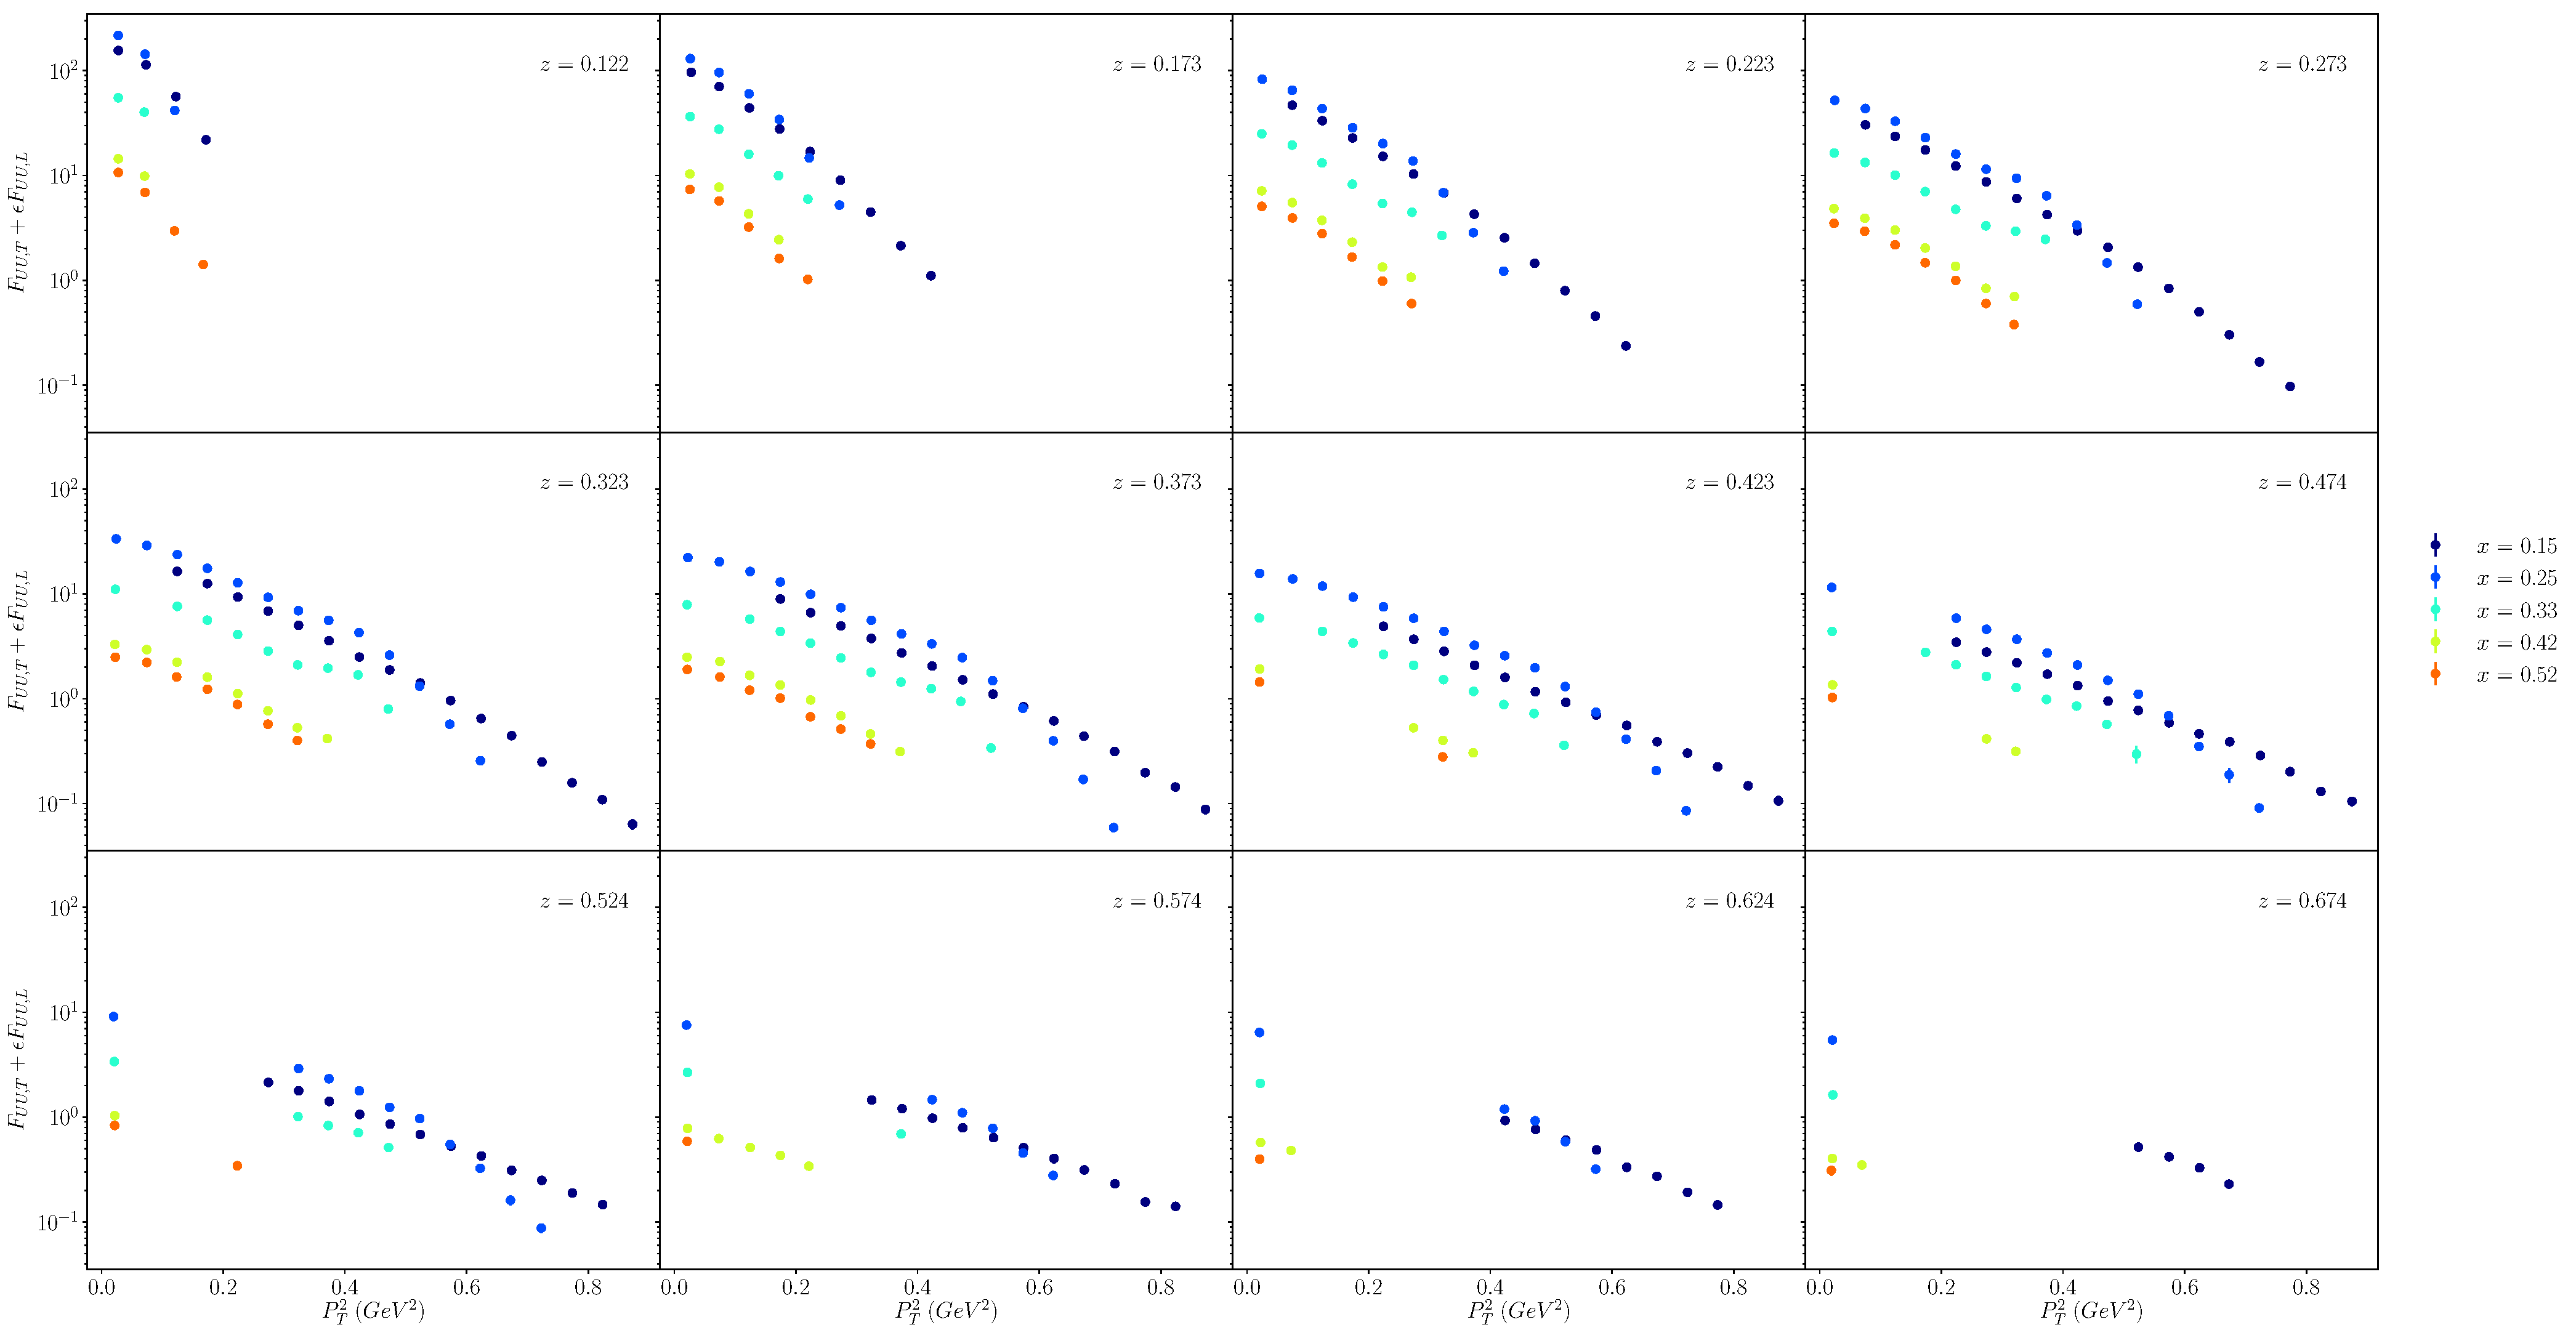
\includegraphics[width = \textwidth]{image/plots/sidis/pip_f0_superimpose_x.pdf}
	\caption{The unpolarized structure functions ($\pi^+$) that don't depend on the angle $\phi_h$ are shown here for different values of $x$, $z$, and $P_T^2$.}
	\label{fig:pipf0x}	
\end{sidewaysfigure}

\begin{sidewaysfigure}
	\centering 
	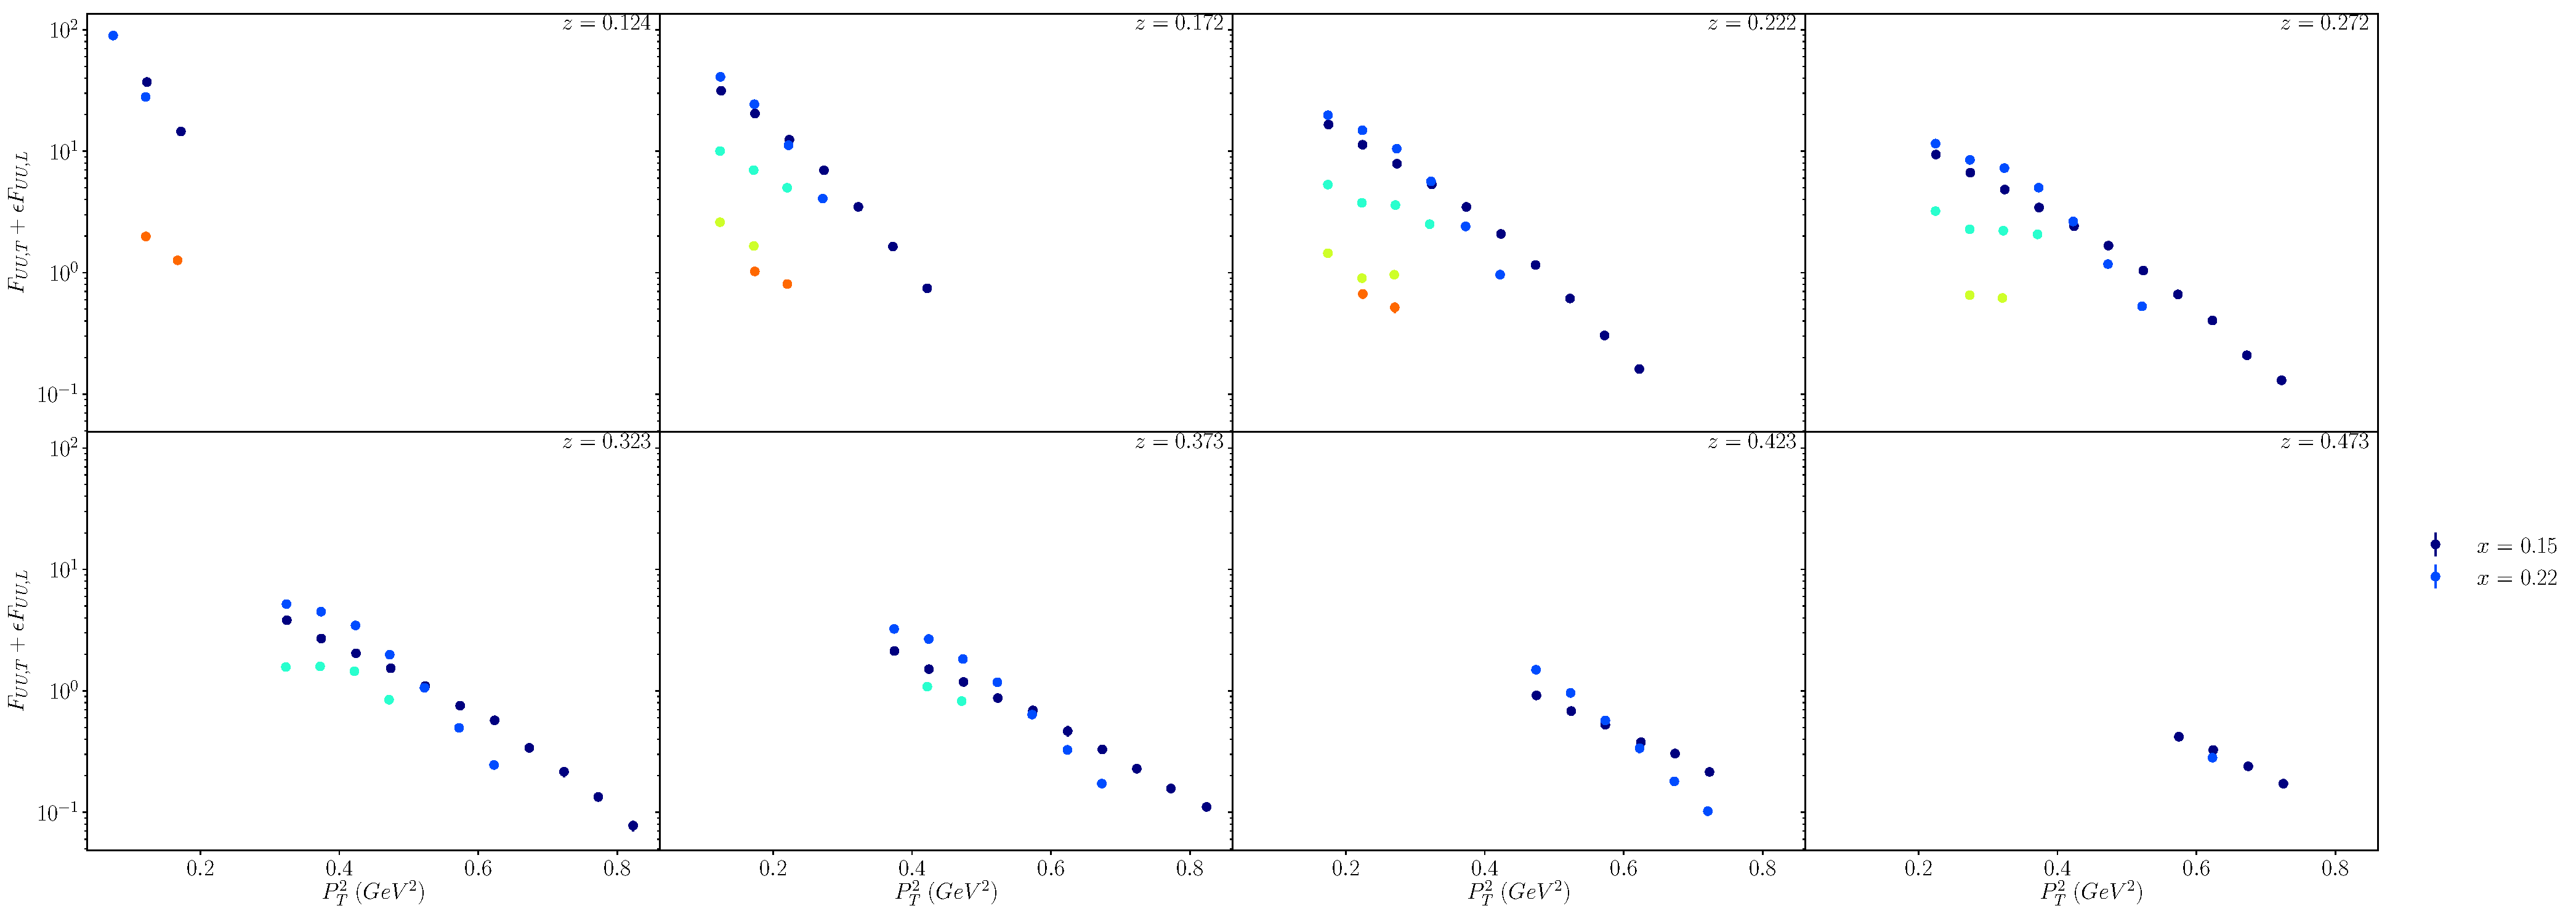
\includegraphics[width = \textwidth]{image/plots/sidis/pim_f0_superimpose_x.pdf}
	\caption{The unpolarized structure functions ($\pi^-$) that don't depend on the angle $\phi_h$ are shown here for different values of $x$, $z$, and $P_T^2$.}
	\label{fig:pipf0x}	
\end{sidewaysfigure}

\begin{sidewaysfigure}
	\centering 
	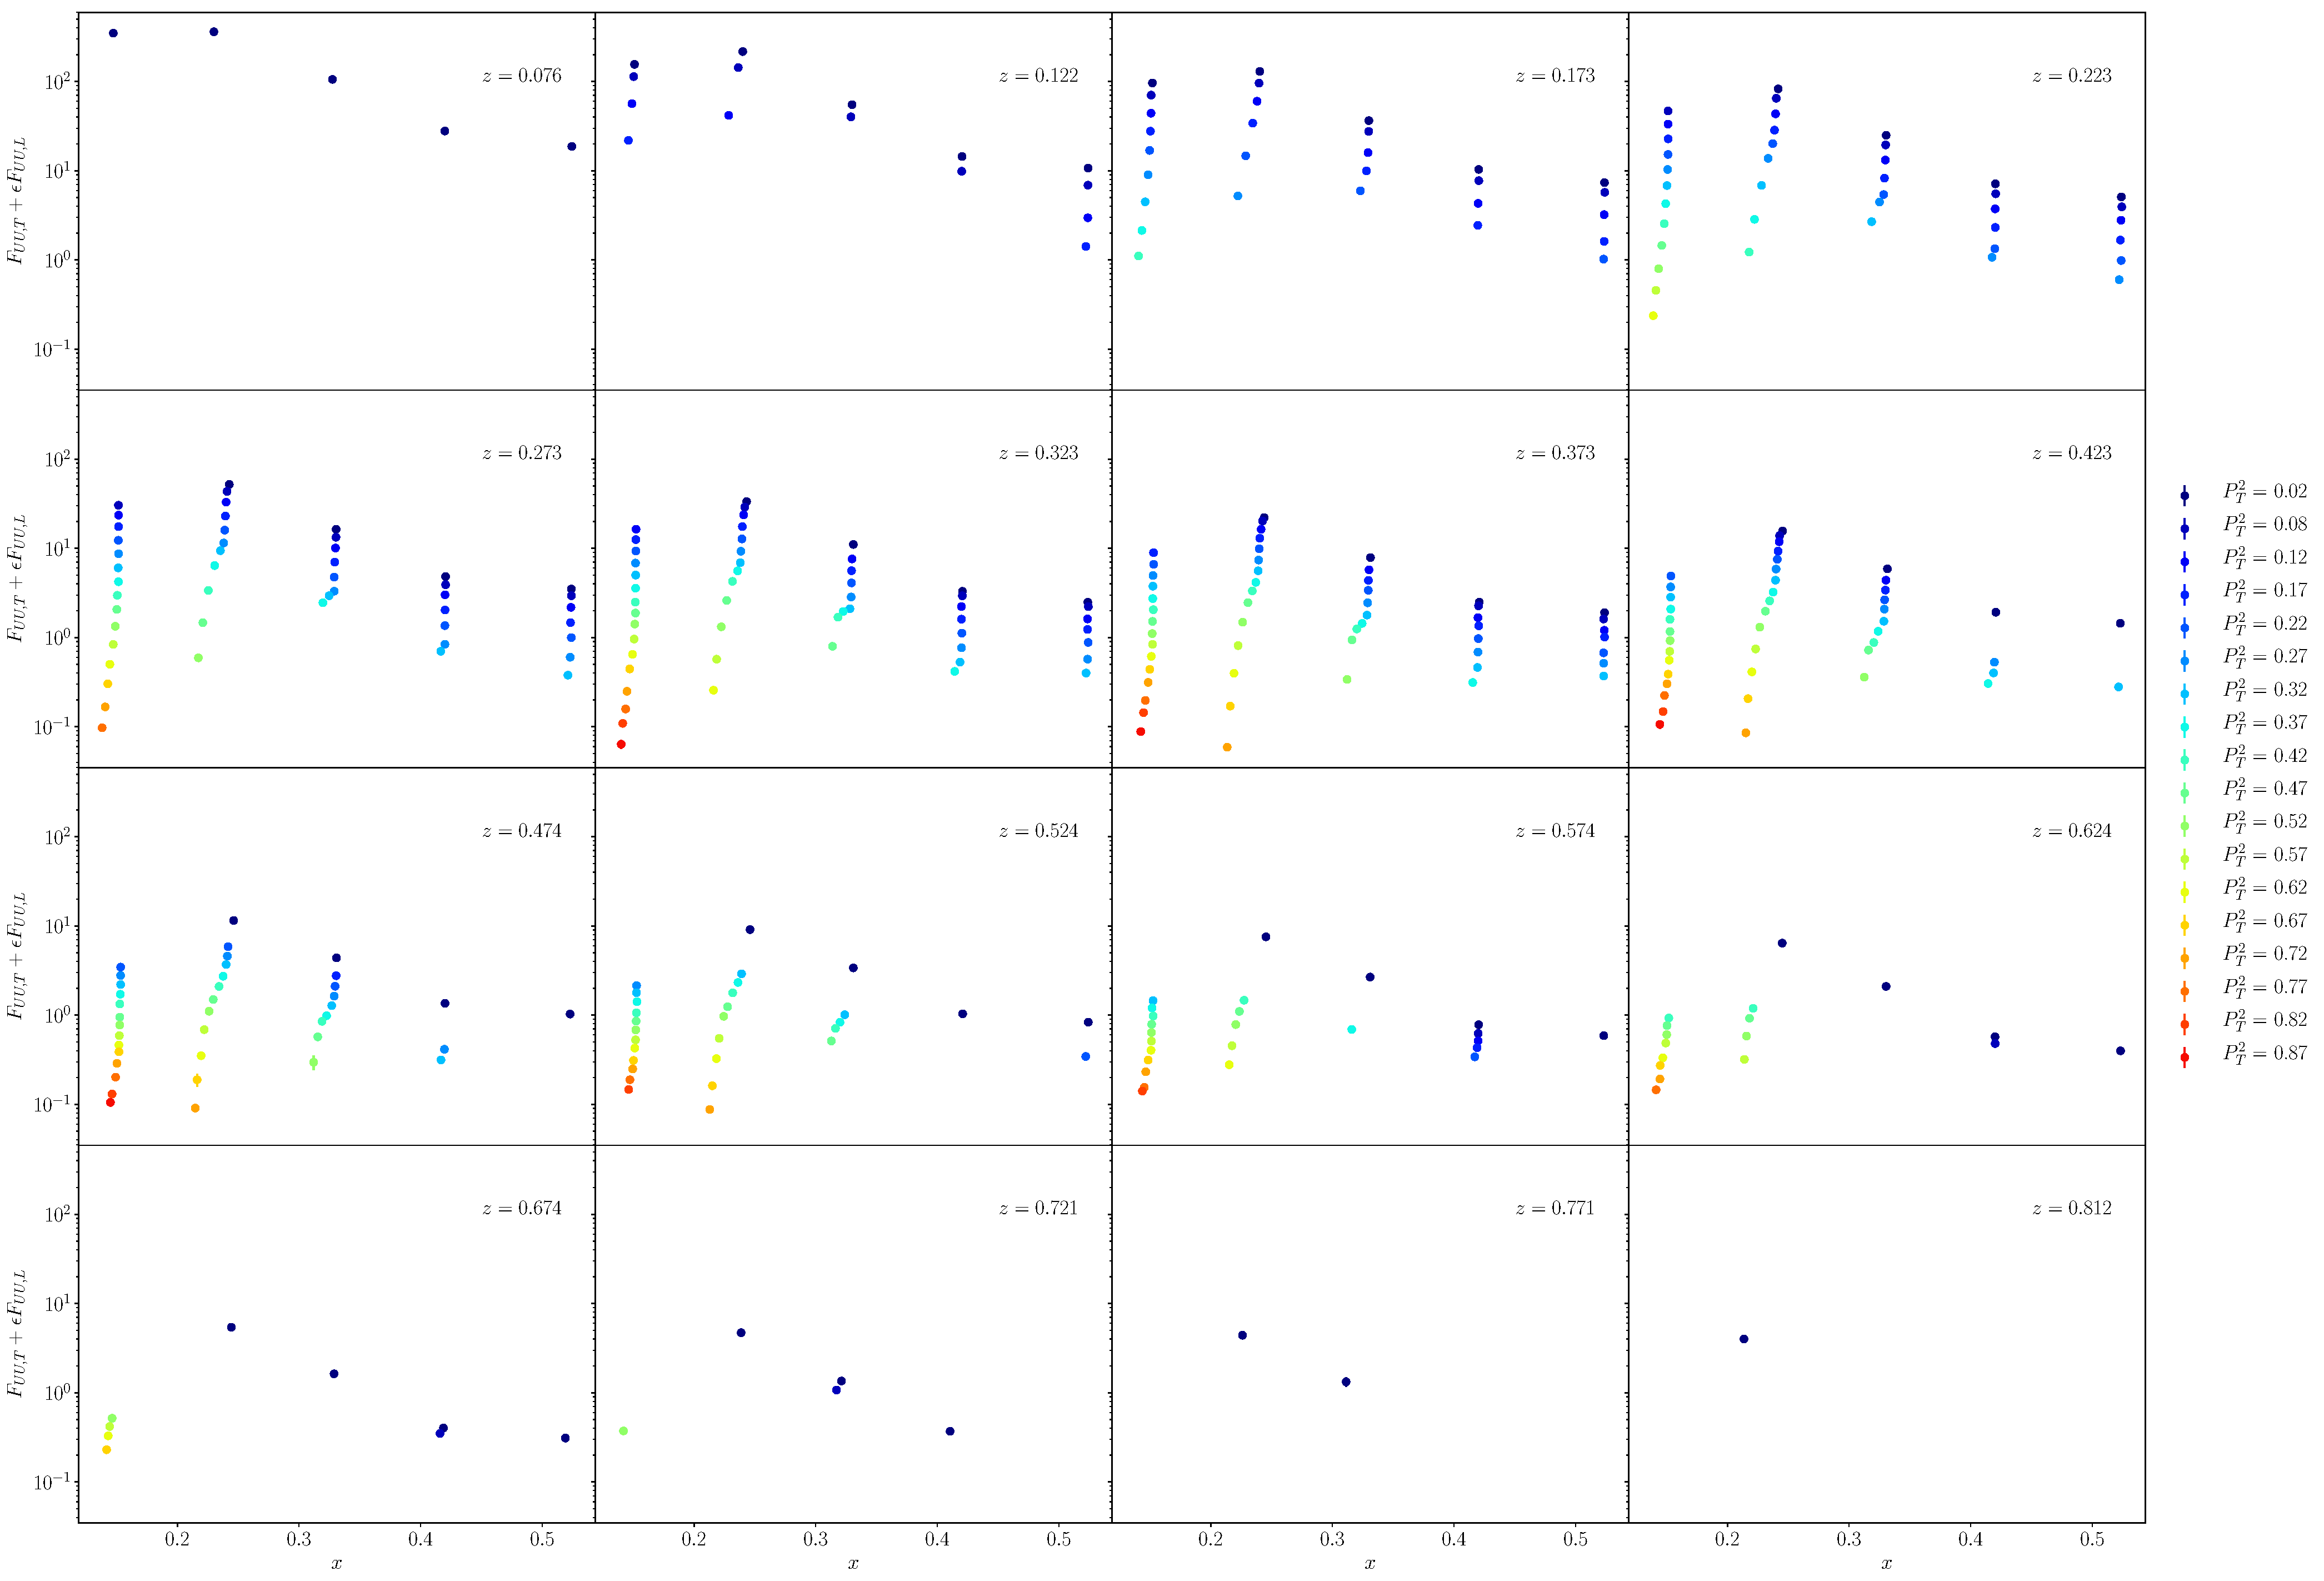
\includegraphics[width = \textwidth]{image/plots/sidis/pip_f0_superimpose_pt2.pdf}
	\caption{The unpolarized structure functions ($\pi^+$) that don't depend on the angle $\phi_h$ are shown here for different values of $x$, $z$, and $P_T^2$.}
	\label{fig:pipf0x}	
\end{sidewaysfigure}

\begin{sidewaysfigure}
	\centering 
	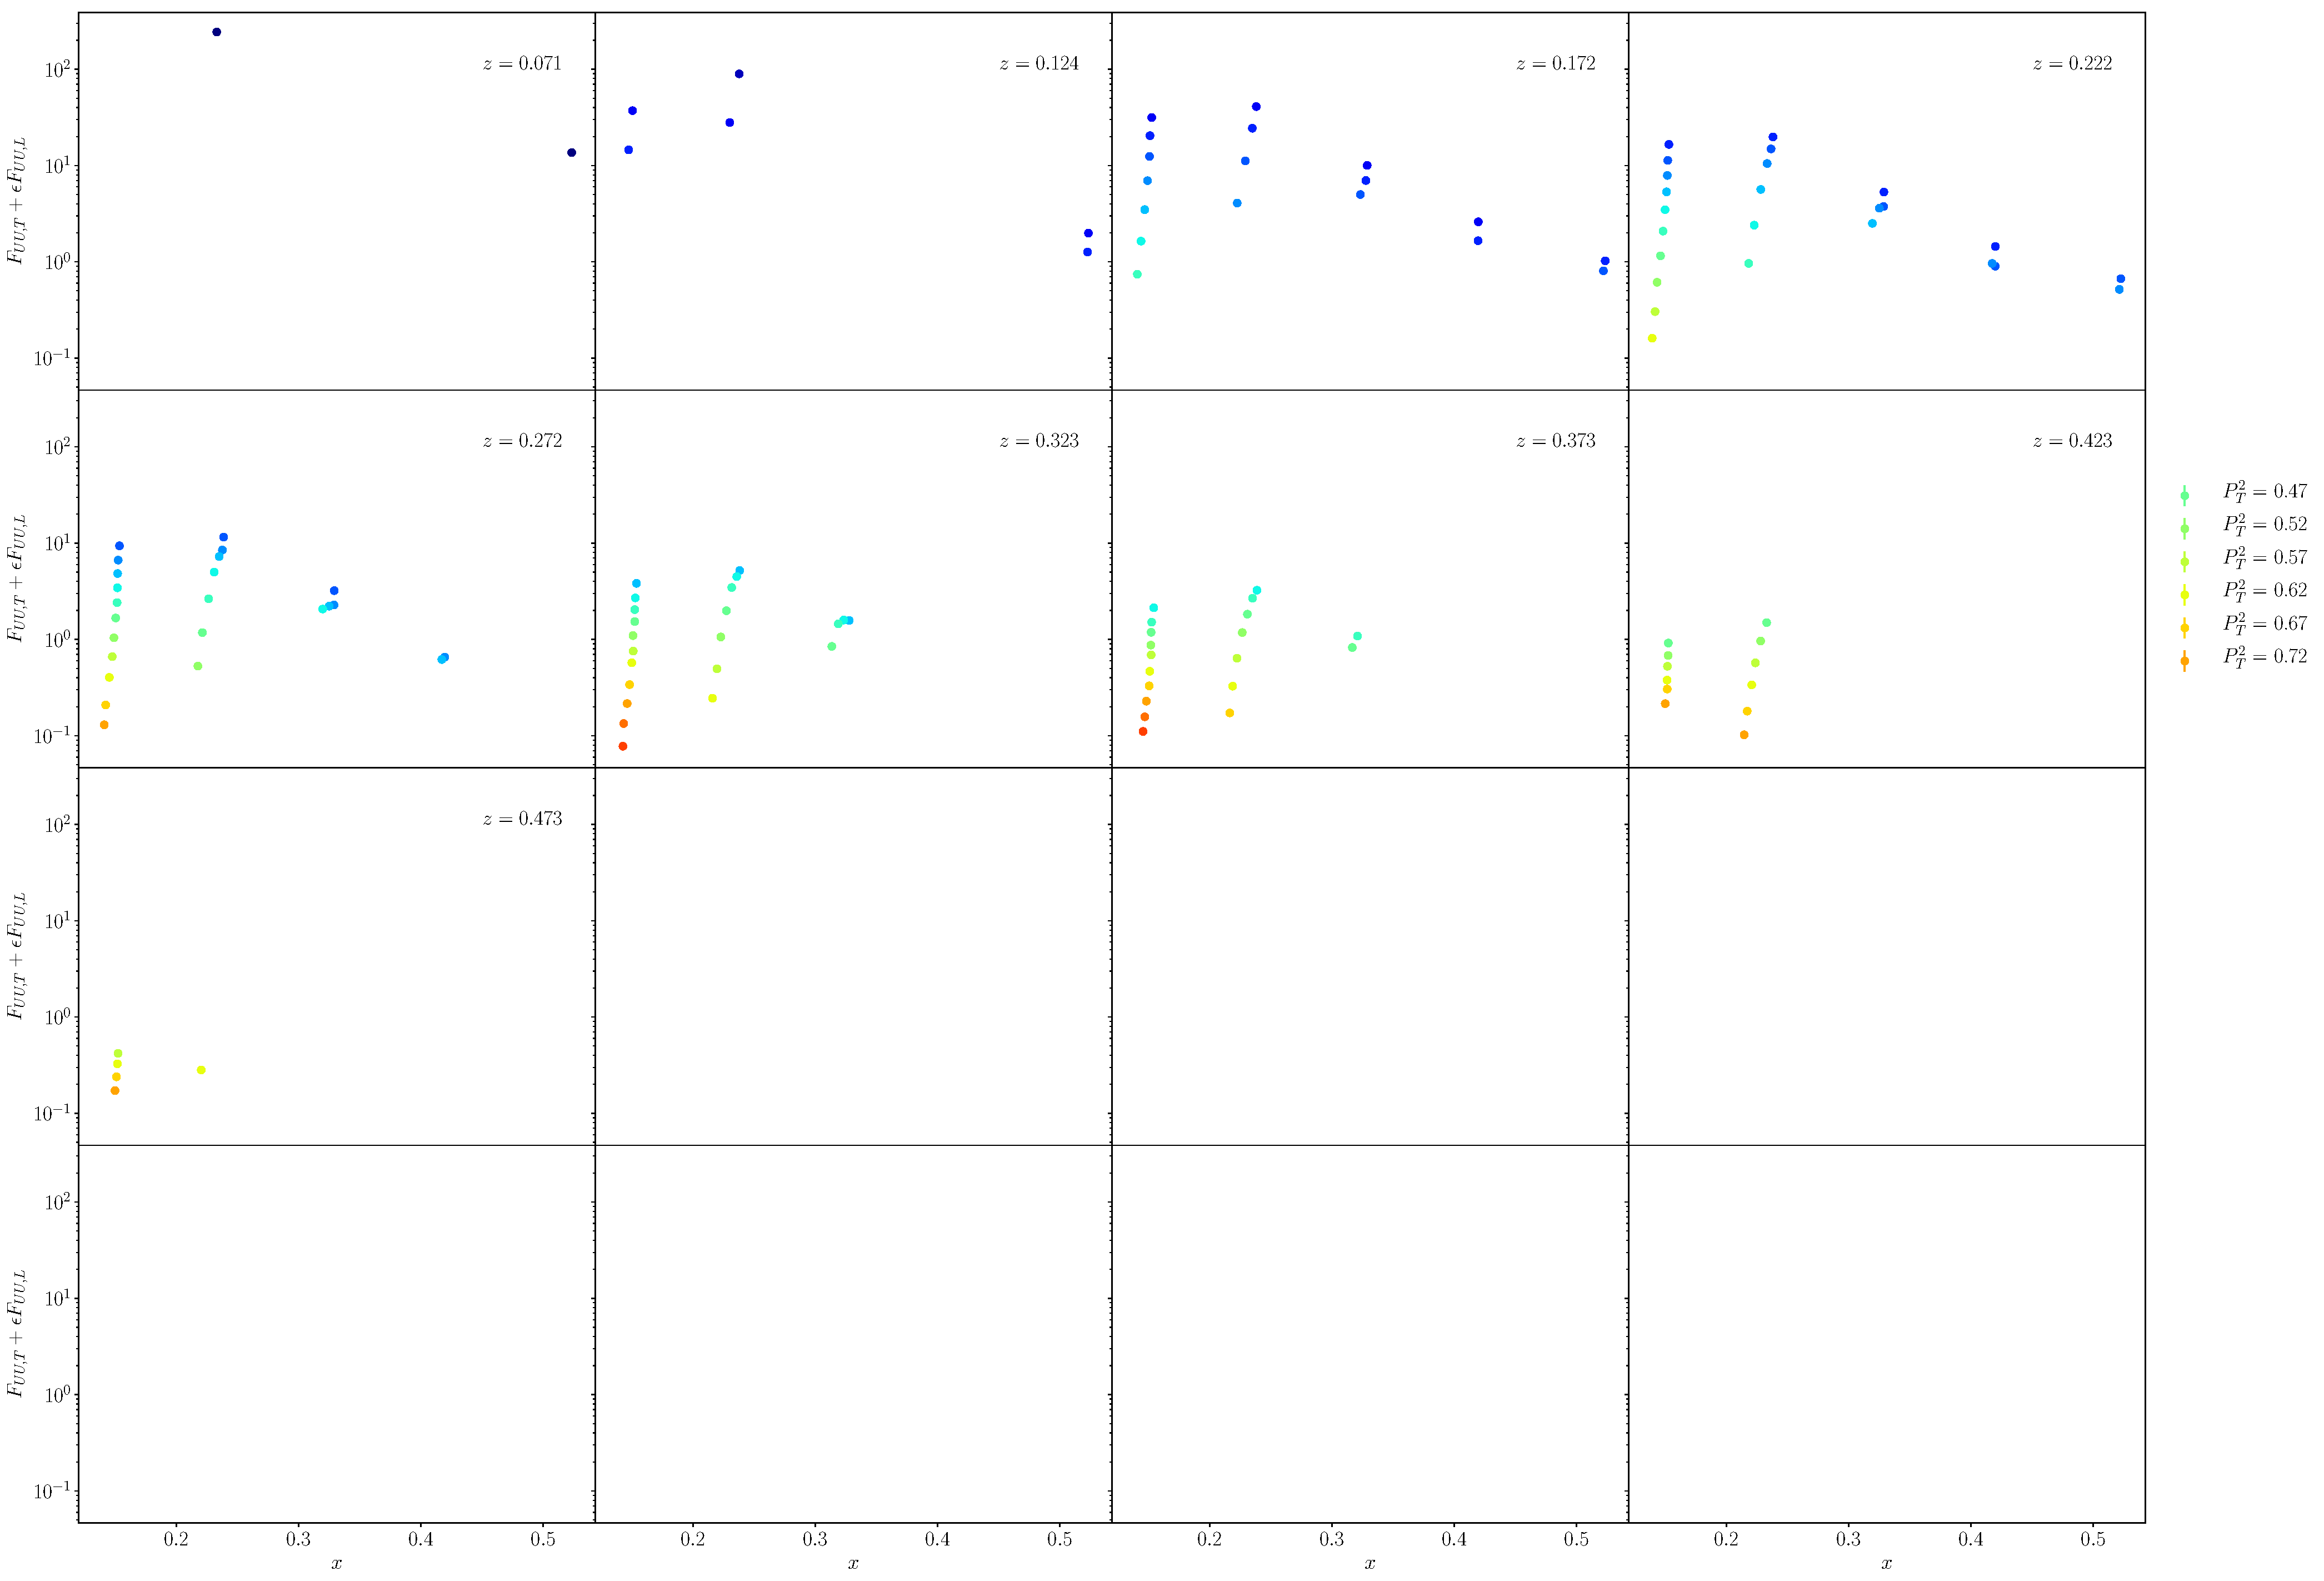
\includegraphics[width = \textwidth]{image/plots/sidis/pim_f0_superimpose_pt2.pdf}
	\caption{The unpolarized structure functions ($\pi^-$) that don't depend on the angle $\phi_h$ are shown here for different values of $x$, $z$, and $P_T^2$.}
	\label{fig:pipf0x}	
\end{sidewaysfigure}
